\chapter{Controllable Fusion Large Language Models and Knowledge Graphs}
\label{chap:controllable_fusion}

% Comment: This chapter focuses on the methodology for controllable fusion using KG paths

While constraining the answer type, as discussed in Chapter~\ref{chap:act_selection}, provides a valuable signal for improving factuality, another powerful approach involves leveraging the explicit relational structure within the Knowledge Graph more directly. This chapter introduces methods based on the core idea of using KG subgraphs - a small part of the KG that contains the entities from the question, answer candidate generated by the LLM, and the shortest paths between them, drawing upon the work presented in \cite{DBLP:journals/corr/abs-2310-02166, salnikovreranking} and subsequent refinements focused on reranking.


The central motivation for this chapter is to move beyond the knowledge concentrated in parameters of the LLM and instead use pathes derived from the Knowledge Graph. This is similar to how people search in knowledge graphs: they go step-by-step, or hop-by-hop, through connected entities to find answer and become sure that entities are really related. Instead of only using LLM's not transparent generation process for factuality, we suggest using the paths that connect entities from question to potential answer entities in the KG. Such paths are good indicator of factual correctness, giving more control and interpretability, because KG path itself gives concrete evidence that supports given answer.

The general pipeline for this fusion strategy, illustrated in Figure~\ref{fig:controllable_fusion:big_pipe}, involves several stages. First, relevant entities are identified within the input question. Second, candidate answers might be generated by an LLM, or potential answer entities are retrieved from the KG, focusing on entities connected to the question entities via relatively short paths. Crucially, features are extracted from these connecting paths (or the surrounding subgraph). These features capture information about the path structure and relations involved. Finally, these subgraph based features are used by a scoring or reranking model to evaluate the correctness of each candidate answer, ultimately selecting the answer best supported by the explicit structure of the Knowledge Graph. This chapter will detail the specific mechanisms developed for implementing this subgraph based fusion method.

\begin{figure}[htb]
    \centering
    \includegraphics[width=\columnwidth]{kg_path_fusion/new_paper_big_pipeline.pdf}
    \caption{The proposed method for reranking language model answers with KGs. The method includes subgraph extraction, features extraction, and various ranker approaches.}
    \label{fig:controllable_fusion:big_pipe}    
\end{figure}

\section{Answer Candidate Generation}
\label{sec:controllable_fusion:answer_candidate_generation}

As the subgraph extraction protocol requires answer candidates, we need a source of distinct answer candidates for each question, but most LLM approaches for QA, such as the one presented by \cite{DBLP:conf/coling/SenAS22-mintaka}, typically use \texttt{Greed Search} and evaluate the top-1 answer, it is important to note that the correct answer may not always be the top candidate. For example, the fine-tuned T5-XL-SSM~\cite{DBLP:conf/emnlp/RobertsRS20} model achieved higher Mean Reciprocal Rank (MRR) scores for our task, indicating that re-ranking could improve the top-1 results. 

Similar to the previous discussed method in Section~\ref{sec:act_selection:initial_answer_candidate_generation} to generate initial answer candidates, we use Diverse Beam Search~\cite{DBLP:journals/corr/VijayakumarCSSL16-diverse-beam-search} to generate an initial list of answer candidates. This candidates will be used for subgraph extraction and features extraction to rank them and get the final answer for the questions.
  
% In this section, we examine each component of the process in detail.
%  Firstly, we generate answer candidates using various LLMs and generate subgraphs, as discussed in Subsection~\ref{sec:subgraph_extract}. Next, in Subsection~\ref{sec:subgraph_features}, we will look at which attributes are used to rank responses.


% We apply {Diverse Beam Search} to the following LLMs: {T5-large-ssm}, {T5-XL-ssm}, {Mistral}, and {Mixtral} with $200$ beams, $20$ beam groups, and a $0.1$ diversity penalty. We extend our previous research~\cite{DBLP:conf/paclic/SalnikovLRNBMP23-originalpaper} by fine-tuning the proposed T5-like models and comparing them to more recent state-of-the-art models like Mistral and Mixtral, which should make our research more applicable to real-world use cases. T5-large-SSM and T5-XL-SSM were reported to be state-of-the-art both in the original Mintaka paper and our previous work, serving as a good baseline for comparison in this study.

% To finetune the T5-like models, we first train them on English questions for $10000$ steps, following the protocols outlined in the original Mintaka paper~\cite{DBLP:conf/coling/SenAS22-mintaka}. For the more state-of-the-art Mistral and Mixtral, we finetune with LoRA and train on English questions by generating the answer candidates with ``\textit{Answer as briefly as possible without additional information. [Question]}''. However, for the T5-like models, despite adhering to these protocols, we could not achieve the reported Hits@1 accuracy in the original paper. Despite this challenge, the main focus of the study is on the reranking aspect of the pipeline. Therefore, this paper's primary contribution is improving our fine-tuned models.

\section{Subgraph Extraction}
\label{sec:controllable_fusion:subgraph_extract}
The main backbone of our approach is the procedure of subgraph extraction. We rely on the information conveyed in the relationships between question-answer pairs to improve the reranking of LLM generations. To further investigate how this relationship can improve performance, we employ a subgraph extraction algorithm that generates a KG's subgraph containing entities relevant to each question-answer pair and the shortest paths between them that contain relevant properties/relationships. 
% We extract various features that can be used for reranking in addition to the subgraphs. This section presents the subgraph extraction algorithm, the features derived from the subgraphs, and our reranking approaches.

\begin{figure}[htb]
    \centering
    \includegraphics[width=\columnwidth]{kg_path_fusion/ssp_to_sub.pdf}
    \caption{The proposed method for reranking language model answers with KGs. The method includes subgraph extraction, features extraction, and various ranker approaches.}
    \label{fig:controllable_fusion:subgraph_construction_example}
\end{figure}

For each question-answer candidate pair, the desired subgraph $G$ is mathematically defined as an induced subgraph of the Knowledge Graph. Thus, given our shortest paths from $e_i~\rightarrow~A$, where $e_i$ - entity extracted from question and $A$ - Answer. We can use the following Listing~\ref{alg:controllable_fusion:sub_extract} to extract $G$. Let us define $H$ as the set of all distinct nodes within our shortest paths $P_i$. We want to preserve all edges between the nodes within $H$. For all question-answer pairs, our objective is to retain the relationship between our question entities $E$ and answer candidate entity $A_i$. The process is schematically depicted at Figure~\ref{fig:controllable_fusion:subgraph_construction_example}.

\begin{ListingEnv}[p]
    \centering % Center the listing if desired
    \caption{Subgraph Extraction Algorithm} 
    \label{alg:controllable_fusion:sub_extract} 
    \begin{lstlisting}[basicstyle=\fontsize{10pt}{12pt}\selectfont\ttfamily] % Smaller font for code Require: entities, candidate

paths = []
For entity in entities:
    shortest_paths = get_shortest_path(entity, candidate)
    paths.extend(shortest_paths)

H = set of unique nodes in paths

G = new Graph()
Add nodes from H to G

For unique_node in H:
    unique_node_neighbors = get_neighbors(unique_node)
    For neighbor_node in unique_node_neighbors:
        If neighbor_node in H:
            Add edge (unique_node, neighbor_node) to G

Return G
    \end{lstlisting}
\end{ListingEnv}


\section{Features based on Extracted Subgraphs}
\label{sec:controllable_fusion:subgraph_features}
After extracting subgraphs for all answer candidates of our LMs, we use all possible useful features for reranking. Referring to our previous study, we mainly focused on a simple text representation of the extracted subgraphs to rank our answer candidates. Thus, in this study, we propose extracting as many useful features as possible and analyzing each feature's importance in this reranking problem. We have divided the features into the following main categories: graph, text, and Graph2Text sequence features. 

\subsection{Graph Features}
\label{sec:controllable_fusion:graph_features}
With our extracted subgraphs and their corresponding answer candidate, we seek to use the relationship from the subgraphs to classify the correct answer candidate. As the first simple baseline, we utilize graph features consisting of simple numerical subgraph statistics. We hypothesize that subgraphs with the correct answer will be less ``complex'' than subgraphs with the incorrect answer candidate. Therefore, we would want the graph features to convey the complexity of the respective subgraph. With a clear objective in mind, we experiment with the following graph features:  

\begin{itemize}
    \item \textbf{Number of nodes and edges}: basic statistics of the nodes and edges of graph $G$.
    \item \textbf{Number of cycles}: a cycle of graph $G$ is a non-empty path that starts from a given node and ends at the same node. 
    \item \textbf{Number of bridges}: a bridge of graph $G$ is an edge, where its deletion increases the number of connection components. 
    \item \textbf{Average shortest path}: the average of each shortest path between the question entity and the answer entity. 
    \item \textbf{Density}: measurement of the density of a graph, where the number of edges in a dense graph is close to the maximal number of edges (each pair of nodes is connected by an edge). The density $d$ for the graph $G$ is formulated as $d = \frac{m}{n(n-1)}$, where $n$ is the number of nodes and $m$ is the number of edges in $G$.
   \item \textbf{Katz centrality}~\cite{katz1953new}: measurement of the importance (or ``centrality'' - how ``central'' a node is in the graph) of a specific node $i$ in a graph $G$. The Katz centrality for node $i$ of graph $G$ is formulated as $x_i = \alpha \sum_{j} A_{ij} x_j + \beta$, where $A$ is the adjacency matrix of graph $G$ with eigenvalues $\lambda$, $\beta$ is the parameter that controls the initial centrality, and $\alpha < \frac{1}{\lambda_{\max}}$. 
    \item \textbf{PageRank}~\cite{page1999pagerank}: a popular algorithm used by Google to rank web pages in the search query by counting the number and quality of links to a page to determine an estimate of its importance. In graph theory, the ``web pages'' and ``links'' are synonymous with nodes and edges. 
\end{itemize}

\noindent We hypothesize that these features may provide ranker models with insights into the complexity of the respective subgraphs.


\subsection{Text Features}
\label{sec:controllable_fusion:text_features} 
The ablation study showcased the importance of including the question within the text representation of the subgraph. Therefore, besides the simple graph features, we want to emphasize each question/answer pair without using extracted subgraphs. Thus, the text features represent the concatenation between the question and answer, separated by a semicolon --- ``\texttt{;}''. To use this simple concatenation for all ranker approaches, we encode the string using the MPNet\footnote{\url{https://huggingface.co/sentence-transformers/all-mpnet-base-v2}} embedding model~\cite{DBLP:conf/nips/Song0QLL20}.


\subsection{Graph2Text Sequence Features}
\label{sec:controllable_fusion:g2t_seq} 
Given the vast amount of data contained in Knowledge Graphs, it is essential to convert this information into natural language to facilitate understanding and accessibility. Converting a graph into text, known as KG-to-text or Graph2Text, has demonstrated notable success in various applications~\cite{DBLP:journals/corr/abs-2309-11206}. Therefore, when generating text from a Knowledge Graph, it is crucial to analyze the underlying graph structure carefully to ensure accurate translation.

Without an obvious way of incorporating the question within the subgraphs, relying purely on the subgraphs to rerank is ineffective~\cite{DBLP:conf/paclic/SalnikovLRNBMP23-originalpaper}. Therefore, we address this issue by further exploration of different KG-to-text methods. The main objective is experimenting with various techniques to represent the extracted subgraphs more explicitly. For this type of textual feature, we researched and developed three methods for representing subgraphs as a text, including \textbf{Graph2Text Deterministic,  Graph2Text T5, and  Graph2Text GAP}.

Firstly, we employ the \textbf{Graph2Text Deterministic} approach, the most straightforward text linearization approach. In simple terms, the subgraphs are unraveled by their matrix representation. Firstly, to linearize, we convert the subgraph into its binary adjacency matrix. Let us call it matrix $A$. 
Given $n$ nodes in the subgraph, the resulting matrix's dimension will be $n \times n$. The matrix's element $[i, j]$ represents the existence of an edge between a node with index $i$ and a node with index $j$. Then, we replace the edges in the matrix with the edge label and call it $A'$. 
Adjacency matrices are typically implemented with graphs with numeric weights. The weights were string representing the relationship between our nodes. Thus, we represented the existence of an edge with $1$, then replaced in the edge with the string relationship.
%Let us call this adjacency matrix with edge information . 
Lastly, we unravel $A'$ row by row to produce our final sequence and add the triple (node\_from, edge, node\_to) to our final sequence. Listing~\ref{alg:controllable_fusion:sub2seq} summarizes the aforementioned steps. 

\begin{ListingEnv}[p]
    \centering % Center the listing if desired
    \caption{Subgraphs to Sequence - Graph2Text Deterministic} 
    \label{alg:controllable_fusion:sub2seq} 
    \begin{lstlisting}[basicstyle=\fontsize{10pt}{12pt}\selectfont\ttfamily] % Smaller font for code

Require: Subgraph G
Ensure: Text representation of subgraph Seq

adj_matrix = get_adjacency_matrix(G)
Seq = ""
# Assuming adj_matrix is n x n, where n is number of nodes
# and indices correspond to node IDs
For i in range(number_of_nodes(G)): 
    For j in range(number_of_nodes(G)):
        # Assuming 0 indicates no edge, non-zero indicates an edge
        If adj_matrix[i][j] != 0: 
            # Assuming G allows lookup by index i, j
            node_i_label = get_node_label(G, i) 
            node_j_label = get_node_label(G, j)
            # Get edge info (label/type) between node i and j
            edge_info = get_edge_info(G, i, j) 
            # Append triple to sequence string, separated by e.g., semicolon
            Seq += node_i_label + " " + edge_info + " " + node_j_label + "; " 
Return Seq
    \end{lstlisting}
\end{ListingEnv}

For the remaining two text linearization approaches, \textbf{Graph2Text T5} and \textbf{Graph2Text GAP}, we employ more complex neural-based models trained on the WebNLG~2.0 dataset~\cite{DBLP:conf/acl/GardentSNP17}. This dataset consists of instances, where each includes a Knowledge Graph from DBpedia~\cite{DBLP:conf/semweb/AuerBKLCI07} and a target text comprising one or more sentences that describe the graph. The test set is divided into partitions of seen (DBpedia categories present in the training set) and unseen (DBpedia categories not present in the training set). The statistics of this hand-crafted and human-verified dataset are described in detail in Table~\ref{tab:controllable_fusion:webnlg_label}. 

\begin{table}
    \centering
    \caption{Statistics of the WebNLG 2.0 parallel knowledge graph-to-text dataset.}
    
    \begin{subtable}[t]{0.48\textwidth}
    \centering
    \begin{tabular}{lr}
        \toprule
        \textbf{Entities} & 2,730 \\
        \textbf{Relations} & 354 \\
        \textbf{Triples} & 81,927 \\
        \bottomrule
    \end{tabular}
    \caption{Knowledge Graph statistics. Total number of KG components, number of tokens in the narratives.}
    \label{tab:kg_stats}
    \end{subtable}
    \hfill
    \begin{subtable}[t]{0.48\textwidth}
    \centering
    \begin{tabular}{lr}
        \toprule
        \textbf{Total} & 623,902 \\
        \textbf{Unique} & 8,075 \\
        \textbf{Entity} & 60\% \\
        \bottomrule
    \end{tabular}
    \caption{Texts statistics. The percentage of text entities represents the portion of the text that includes entity labels.}
    \label{tab:controllable_fusion:webnlg_label}
    \end{subtable}
\end{table}

The idea behind the \textbf{Graph2Text T5} approach is to extract informative and useful features from KGs using pre-trained text-to-text LMs. With the impressive capabilities of pretrained LMs in the text-to-text generation task, we seek to replicate such results in the graph-to-text scope. Our idea is built upon the analogous algorithm discussed in~\cite{DBLP:journals/corr/abs-2007-08426}. The authors tackle the graph-to-text generation task in this work with two popular text-to-text pre-trained LMs, BART and T5. These models have an encoder-decoder architecture, which makes them well-suited for conditional text generation tasks. To adapt these models for the graph-to-text task, the authors continue pre-training BART and T5 using the following approaches:

\begin{enumerate}
    \item Language Model Adaptation (LMA): the models are trained on reference texts that describe graphs, following the BART and T5 pre-training strategies.
    \item Supervised Task Adaptation (STA): the models are trained on pairs of graphs and their corresponding texts collected from the same or a similar domain as the target task --- graph-to-text in this case. 
\end{enumerate}

Building on the STA approach via T5 and WebNLG~2.0, we obtain graph-to-text sequences by first converting the graph into a sequence of tokens through linearization. We use the string ``convert the [graph] to [text]:'' to acquire this linearised sequence. This output sequence is then fed into the input sequence for the T5 model tuned on WebNLG~2.0. 
% For tuning Graph2Text T5 approach, we use the following hyperparameters: \textit{learning rate}: $1e^{-3}$, \textit{batch size}: 4, \textit{gradient accumulation steps}: 32, and \textit{Adam optimizer}. 

The \textbf{Graph2Text GAP} approach is based on the current state-of-the-art graph-to-text task, GAP, built on BART~\cite{DBLP:conf/coling/ColasAW22-GAP}. 
The main idea of GAP is a fully graph-aware encoding combined with the coverage of pre-trained LMs. The GAP KG-to-text framework fuses graph-aware elements into existing pre-trained LMs, capturing the advantages brought forth by both model types. The architecture of this solution consists of two main components:

\begin{enumerate}
\item \textbf{Global Attention}: to capture the graph's global semantic information, the graph's components are first encoded using an LM. This allows the model to leverage the lexical coverage of pre-trained LMs.
\item \textbf{Graph-aware Attention}: to attend to and update the representations of entities, relations, or both, a topological-aware graph attention mechanism was introduced, which includes entity and relation type encoding.
\end{enumerate}

Applying the work of GAP, we first linearize the input graph into a text string by creating a sequence of all triples in the KG, interleaved with tokens that separate each triple and the triple's components (head, relation, and tail). Then, we use a transformer encoder to obtain vector representations. The first module in each transformer layer acts as a Global Attention and captures the semantic relationships between all tokens. Moreover, we use a Graph-aware Attention module to capture the sparse nature of adjustment in a graph and apply it to entity and relation vectors from word vectors. By proposing this flexible framework, where graph-aware components can be interchanged, the current architecture aims to generate coherent and representative text descriptions of the KG. Like the Graph2Text T5 approach, we pretrain the model on the WebNLG~2.0 dataset and get the final predictions through the fine-tuned model. 
% For finetuning the Graph2text GAP approach, we use the following hyperparameters: \textit{learning rate}: $2e^{-5}$, \textit{batch size}: 16; \textit{beam size}: 5, \textit{Adam Optimizer}, 50 \textit{nodes}, and 60 \textit{relations}.


In this research, we introduce the more complex neural-based graph-to-text approach to explore further the reranking capabilities of the textual representation of our extracted subgraphs. The initial rudimentary text linearization approach has already achieved state-of-the-art Hits@1. We look for a more complete case study on reranking the text linearization with these two neural-based linearization approaches. To better understand the differences between these methods, we present several illustrative examples that demonstrate how T5 and GAP handle different types of knowledge graph structures.

Let us examine four representative examples that highlight the key differences in how these models process and represent graph information presented in on Figures~\ref{fig:controllable_fusion:g2t_example1},~\ref{fig:controllable_fusion:g2t_example2},~\ref{fig:controllable_fusion:g2t_example3}, and~\ref{fig:controllable_fusion:g2t_example4}:

\begin{figure}[!htb]
    \centering
    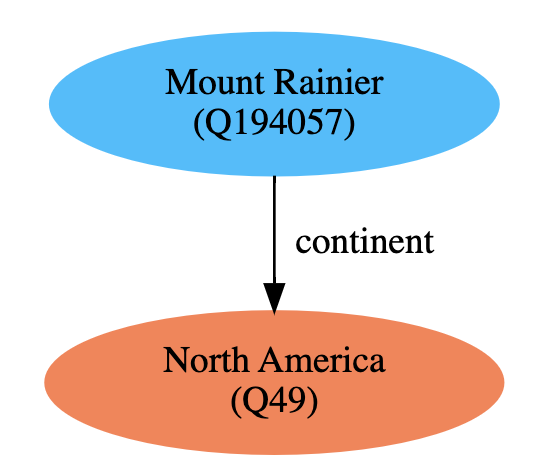
\includegraphics[width=0.5\textwidth]{kg_path_fusion/g2t_examples/g2t_e1.png}
    \caption{Example 1: Simple location relationship between Mount Rainier and North America. The T5 model correctly states ``Mount Rainier is located in North America,'' while GAP introduces an incorrect inference by stating ``The summit of North America is called Mount Rainier.''}
    \label{fig:controllable_fusion:g2t_example1}
\end{figure}

\begin{figure}[!htb]
    \centering
    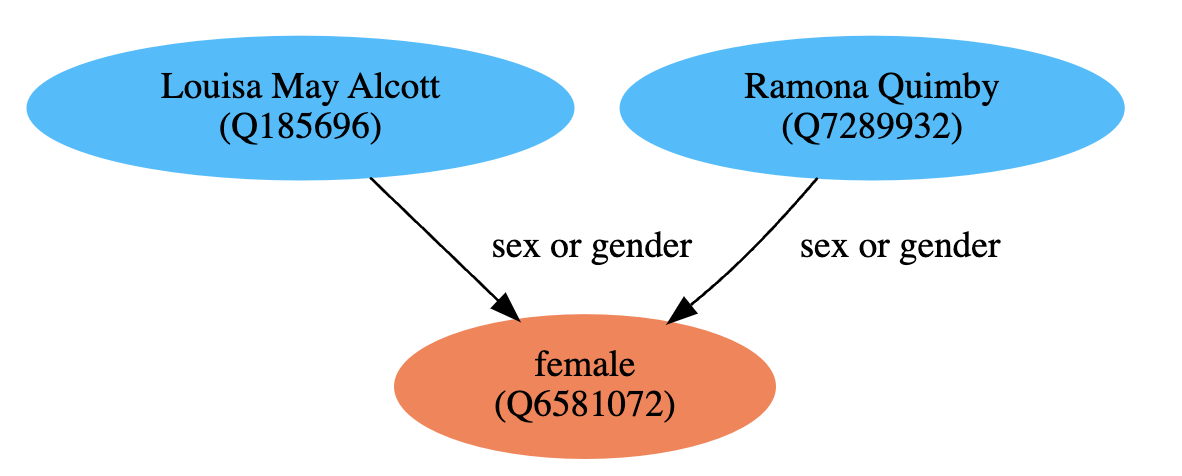
\includegraphics[width=0.6\textwidth]{kg_path_fusion/g2t_examples/g2t_e2.png}
    \caption{Example 2: Gender information for two authors. The T5 model accurately states ``Louisa May Alcott and Ramona Quimby are both females,'' while GAP makes a significant error by stating they are ``both men,'' demonstrating a critical failure in preserving factual information.}
    \label{fig:controllable_fusion:g2t_example2}
\end{figure}

\begin{figure}[!htb]
    \centering
    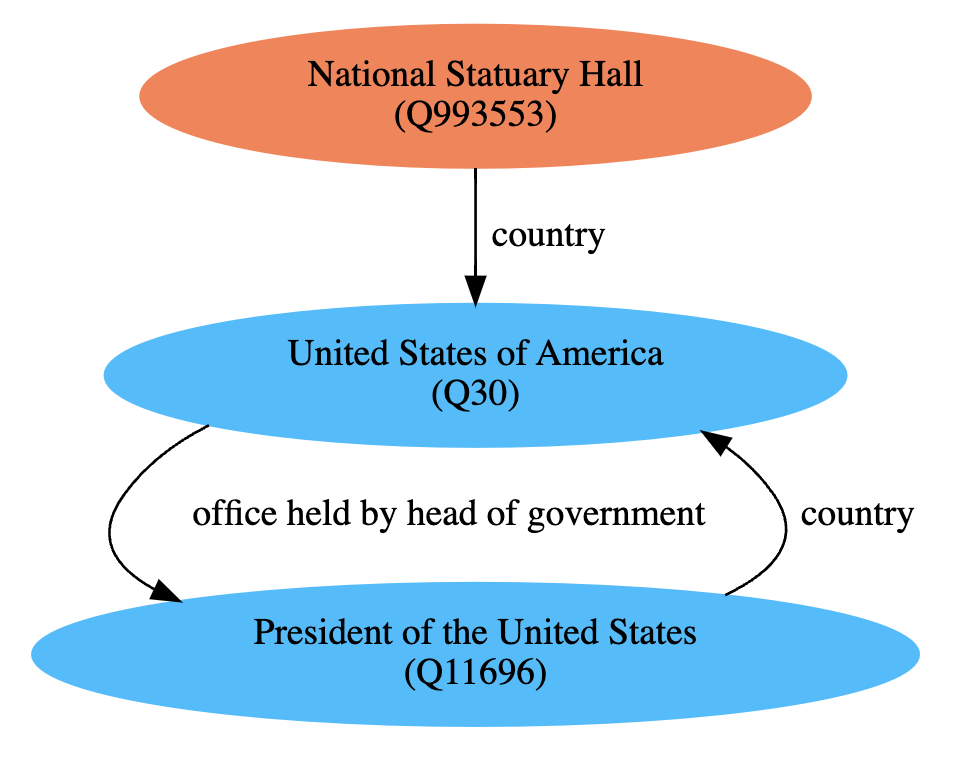
\includegraphics[width=0.6\textwidth]{kg_path_fusion/g2t_examples/g2t_e3.png}
    \caption{Example 3: Complex relationships involving the United States and its institutions. The T5 model provides a clear and accurate description: ``The United States of America is the location of the National Statuary Hall and the office of the President of the United States.'' In contrast, GAP generates a more verbose and less precise description, introducing unnecessary information about Congress and creating redundant statements about the presidency.}
    \label{fig:controllable_fusion:g2t_example3}
\end{figure}

\begin{figure}[!htb]
    \centering
    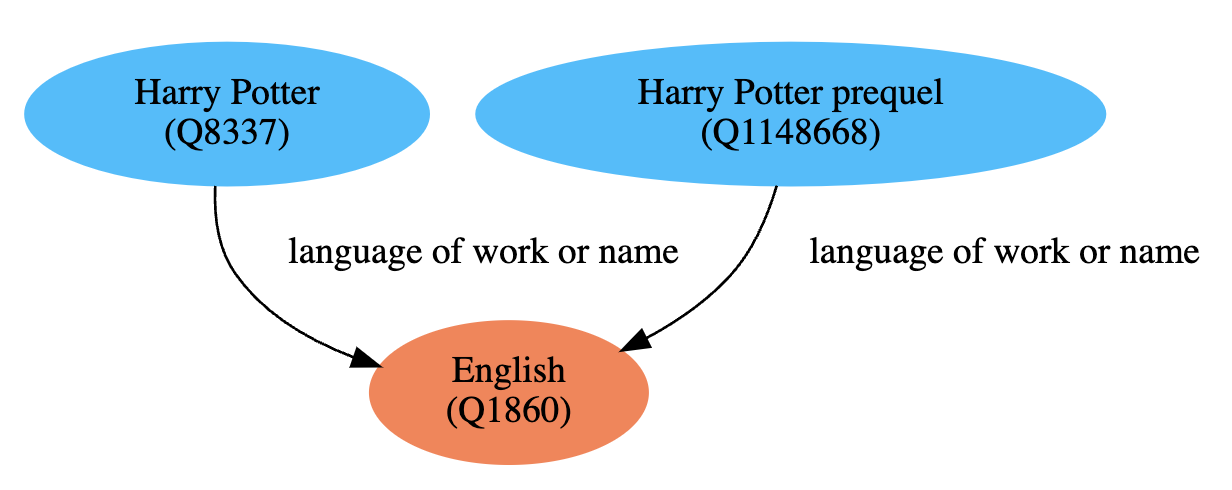
\includegraphics[width=0.6\textwidth]{kg_path_fusion/g2t_examples/g2t_e4.png}
    \caption{Example 4: Language information for Harry Potter works. The T5 model correctly states ``The Harry Potter prequel is written in English, as is the Harry Potter book,'' while GAP makes an error by referring to ``the English book'' instead of ``the Harry Potter book,'' demonstrating a tendency to lose specific entity information.}
    \label{fig:controllable_fusion:g2t_example4}
\end{figure}

These examples reveal several important patterns in how the two models handle graph-to-text conversion:

\begin{enumerate}
    \item \textbf{Factual Accuracy}: T5 consistently maintains higher factual accuracy, while GAP occasionally introduces incorrect inferences or loses specific entity information.
    
    \item \textbf{Information Preservation}: T5 better preserves the specific details from the knowledge graph, whereas GAP tends to generalize or introduce unnecessary information.
    
    \item \textbf{Conciseness}: T5 generates more concise and focused descriptions, while GAP often produces more verbose output with redundant information.
    
    \item \textbf{Entity Handling}: T5 demonstrates better handling of entity relationships, while GAP sometimes confuses or misrepresents entity attributes.
\end{enumerate}

These observations align with our quantitative findings presented in Table~\ref{tab:controllable_fusion:g2t_accuracy}, where T5 shows superior performance in preserving both question and answer entities. The examples particularly highlight GAP's tendency to introduce hallucinations and lose specific entity information, which explains its lower accuracy scores in our evaluation.

% All three variations of Graph2Text Sequence features are further encoded with the MPNet embedding model~\cite{DBLP:conf/nips/Song0QLL20}, discussed more in \ref{appx:detailed_results}. Moreover, motivated by our previous research, we employ context and highlight these Graph2Text sequences, discussed further in \ref{hl_context}.


\section{Rank LLM answer candidates using subgraphs} \label{sec:controllable_fusion:ranker}
With the subgraphs and their extracted features discussed above, we devise several reranking approaches to maximize the performance of the base large language models. As the focal point of the research is the reranking scope, we employ reranking methodologies from least to most complex. The hypothesis is a positive trend in performance as we apply more complex models and features.

As a starting point, we employ semantic reranking. This is a popular solution in information retrieval~\cite{DBLP:journals/jifs/FigueroaPP20, DBLP:journals/corr/HendersonASSLGK17}, implemented differently under the same name. Building on this foundation, our semantic ranker utilizes the MPNET~\cite{DBLP:conf/nips/Song0QLL20} embeddings of the answer candidates, further justified in~\ref{mpnet_explain}. We then rank the answer candidates by the cosine similarity between the embedding vectors. 

In the next layer of complexity, we utilize regression-based models, namely, linear and logistic regression. %~\cite{legendre1806nouvelles}
For the features set, we apply all features discussed in~\ref{sec:controllable_fusion:subgraph_features} (for features in text/string format, we apply MPNET embeddings, discussed in~\ref{mpnet_explain}). In the case of linear regression, we employ ordinary least squares linear regression to predict either $1$ or $0$, corresponding to correct and incorrect responses, respectively. The predicted score was then used to rank the potential answers by sorting the values from highest to lowest. Although we employ logistic regression for the same reranking task, we reformat the problem to a classic classification problem. We sort the answers with the highest classification confidence to rank the candidates. We use a standard logistic regression model with L2 regularisation. 

In addition to regression-based models, we want to utilize the same features with a more complex ranker. Thus, we explore and experiment with the gradient boosting model, specifically the CatBoost regression model~\cite{DBLP:conf/nips/ProkhorenkovaGV18-catboost}. Before training, we use grid search to finetune \textit{learning\_rate, depth,} and \textit{iteration}. We use root-mean-square deviation (RMSE) to evaluate. Like linear regression, we use the predicted score to rank the answer candidates by sorting the values. 

Last but not least, the most effective and complex approach for reranking answer candidates is a neural-based ranker with textual features as input. We experiment with a transformer-based model with an additional regression head layer, which is fine-tuned using {mean-square loss} and {AdamW} optimisation~\cite{DBLP:conf/iclr/LoshchilovH19-adamw}. To keep the experiments clear and transparent, we keep the same MPNet model for this ranker. We employ this variation of sentence transformer throughout this research for various sentence/text embeddings, as mentioned in~\ref{mpnet_explain}. Due to the lack of a straightforward method for utilizing numeric or table-like features with this ranker, we choose not to apply graph features. 


\section{Experiments}
In this section, we describe an experimental setup to test the usability of our proposed language model reranking methods based on KGs. We explore the impact of different combinations of features on reranking performance and examine the effects of various reranking methods, ranging from simple to more sophisticated, on reranking accuracy.

\subsection{Dataset} \label{sec:dataset}
To further enhance the results gathered in the original paper, we also conduct our research on Mintaka~\cite{DBLP:conf/coling/SenAS22-mintaka} dataset, which is a large-scale, complex and natural dataset that can be used for end-to-end question-answering models, composed of $20,000$ question-answer pairs. This dataset is annotated with Wikidata entities and comprises 8 types of complex questions. These types include: 
\begin{itemize}%[noitemsep]
    \item \textbf{Count}, e.g., Q: How many astronauts have been elected to Congress? A: 4.
    \item \textbf{Comparative}, e.g., Q: Is Mont Blanc taller than Mount Rainier? A: Yes.
    \item \textbf{Superlative}, e.g., Q: Who was the youngest tribute in the Hunger Games? A: Rue.
    \item \textbf{Ordinal}, e.g., Q: Who was the last Ptolemaic ruler of Egypt? A: Cleopatra.
    \item \textbf{Multi-hop}, e.g., Q: Who was the quarterback of the team that won Super Bowl 50? A: Peyton Manning.
    \item \textbf{Intersection}, e.g., Q: Which movie was directed by Denis Villeneuve and stars Timothee Chalamet? A: Dune.
    \item \textbf{Difference}, e.g., Q: Which Mario Kart game did Yoshi not appear in? A: Mario Kart Live: Home Circuit.
    \item \textbf{Yes/No}, e.g., Q: Has Lady Gaga ever made a song with Ariana Grande? A: Yes.
    \item \textbf{Generic}, e.g., Q: Where was Michael Phelps born? A: Baltimore, Maryland.
\end{itemize}

Factoid questions can sometimes have answers that cannot be linked to an entity in knowledge bases (count and yes/no questions). To handle this edge case in a production system, one could first train a classifier to categorize questions into three types: yes/no, count, and other. For this classification task, we train the MPNet (all-mpnet-base-v2)~\cite{DBLP:conf/nips/Song0QLL20} model using CrossEntropy loss. The training is performed over $5$ epochs on the Mintaka train split, utilizing a batch size of $32$, $500$ warm-up steps, a weight decay of $0.01$, and a learning rate of $0.00005$. To manage the training data, we employ the HuggingFace basic Trainer along with a Weighted Random Sampler. This approach achieves a balanced accuracy of \textbf{98.29\%} on the Mintaka test split.

This research centers around the reranking aspect of the pipeline, discussed in our previous research~\cite{DBLP:conf/paclic/SalnikovLRNBMP23-originalpaper}. Thus, with the question types listed above, we exclude {Yes/No} and {Count} questions. These question types offer no value information, as numbers and yes/no have no respective Wikidata entities, leading to a non-existent/impractical relationship between the question/answer pair. Thus, we deem {Yes/No} and {Count} pointless in the scope of our research. However, one could still utilize the entire pipeline to compute and evaluate the results based on the whole Mintaka dataset, including {Yes/No} and {Count}. 
% Referring to the question type classifier introduced in our original research ~\cite{DBLP:conf/paclic/SalnikovLRNBMP23-originalpaper}, this additional component allows for {Yes/No} and {Count} questions to receive special treatment.

We also compile and publish\footnote{\url{https://github.com/s-nlp/subgraph_kgqas-nlp/KGQA_Subgraphs_Ranking}} the dataset of subgraphs for the whole Mintaka dataset (for train, validation, and test splits separately). Additionally, we also publish the answer candidates generated by the base LMs. Subgraphs are collected using the process discussed in Section~\ref{sec:controllable_fusion:subgraph_extract}: we generate candidate answers, we take the true answer and the entities from the question entity neighbors as candidates, and construct subgraphs with Algorithm~\ref{alg:controllable_fusion:sub_extract}. As a result, we construct a ``correct'' subgraph containing the correct highlighted answer and several ``incorrect'' subgraphs from the incorrect candidate answers generated by the model. 
We present four versions of the dataset with subgraphs: with candidates generated by {T5-Large-SSM}, {T5-XL-SSM}, {Mistral}, and {Mixtral} models.

\subsection{Question Entities} \label{ques_ent}
Referencing the subgraph extraction protocol discussed in~\ref{sec:controllable_fusion:subgraph_extract}, we require question entities and the answer entity for each question-answer pair. Regarding the question entities, any entity linker such as {mGENRE}~\cite{decao2021multilingual} could be applied. However, with the objectives outlined above, utilizing an entity linker would derail the main focus of evaluating this reranking scope. As a result, we leverage the golden truth question entities provided by the Mintaka dataset. 

\subsection{Text Embeddings} \label{mpnet_explain}
Some features derived from the extracted subgraphs are in their natural language form (answer candidates for semantic ranker, Graph2Text sequences, and text features). Therefore, we use these features for our reranking objectives based on the MPNet embedding model~\cite{DBLP:conf/nips/Song0QLL20}. In Performance Sentence Embeddings (evaluation of the quality of the embedded sentence) and Performance Semantic Search (evaluation of the quality of the embedded search queries \& paragraph), the MPNet Embedding model outperforms 37 other sentence transformer models~\cite{reimers-2019-sentence-bert}. These models were compared by averaging the Performance Sentence Embeddings and Performance Semantic Search while considering the speed and the model size. In addition to the highest embedding performance, MPNet is relatively small while fast in training time. Moreover, this model is very popular within the HuggingFace community \footnote{\url{https://huggingface.co/sentence-transformers/all-mpnet-base-v2}}. Utilizing a well-known and widespread embedding model would enhance the aim of formulating our approach as a reranking problem motivated by end-user requirements. 

\subsection{Graph2Text with Highlight \& Context} \label{hl_context}
As mentioned in~\ref{sec:controllable_fusion:g2t_seq}, we focus on different text representations of the subgraphs to rank the respective answer candidates. 
We employ context for linearised text representation of the subgraph. This addition is a simple concatenation between the question and the linearised sequence, separated by a special token $<$/s$>$ to emphasize the question in the question-answer pairing. Moreover, the study showcased the effectiveness of highlighting~(HL) the answer candidate within the linearised sequence of the concatenation. 
The context is motivated by the assumption that the subgraph alone does not provide the necessary information to answer the question. In other words, the model cannot answer the question without it. Similarly, it is difficult to rank the answers if the model has no idea which entities in the subgraph are potential answer candidates.
% With this highlighting scheme, we increased the {Hits@1} by $2\%$, from $0.36 \rightarrow 0.38$ \cite{DBLP:conf/paclic/SalnikovLRNBMP23-originalpaper}. 
An example of such concatenation, the rank by MPNet to achieve the current state-of-the-art, is shown below:  

\begin{itemize}
    \item \textbf{Question}: Which actor was the star of Titanic and was born in Los Angeles, California?
    \item \textbf{Answer}: Leonardo DiCaprio
    \item \textbf{Sequence with HL and Context}: Which actor was the star of Titanic and was born in Los Angeles, California? $<$/s$>$ [unused1]Leonardo DiCaprio[unused2], place of birth, Los Angeles, Titanic, cast member, [unused1]Leonardo DiCaprio[unused2]
\end{itemize}

\noindent We employ a similar \textbf{HL} and \textbf{context} protocol to our three Graph2Text sequences. The objective is to assist the model in understanding the question-answer pair and the Graph2Text sequence. An example of such processing for the three sequences can be seen below:

\begin{itemize}
    \item \textbf{Question}: Which actor was the star of Titanic and was born in Los Angeles, California?
    \item \textbf{Answer}: Leonardo DiCaprio
    \item \textbf{Graph2Text Deterministic}: Which actor was the star of Titanic and was born in Los Angeles, California? $<$/s$>$ [unused1]Leonardo DiCaprio[unused2], place of birth, Los Angeles, Titanic, cast member, [unused1]Leonardo DiCaprio[unused2]
    \item \textbf{Graph2Text T5}: Which actor was the star of Titanic and was born in Los Angeles, California?$<$/s$>$ Los Angeles born [unused1]Leonardo DiCaprio [unused2], who played the role of Jack Sparrow in the film Titanic, was born in the United States.
    \item \textbf{Graph2Text GAP}: Which actor was the star of Titanic and was born in Los Angeles, California?$<$/s$>$Born in Los Angeles, the actor, [unused1]Leonardo DiCaprio [unused2], was a member of the crew of the Titanic.
\end{itemize}

\noindent It is important to note that we employ the \textbf{context} and \textbf{HL} approaches only for the MPNet approach, discussed in Section~\ref{sec:controllable_fusion:ranker}. Sensibly, the transformer-based model trained on sentences and paragraphs is adept at extracting useful information from natural texts. Thus, unlike our other proposed approaches, the MPNet approach classically only handles text embedding as input. Therefore, we utilize \textbf{context} and \textbf{HL} to give the model the best chance at extracting useful information to rank answer candidates. Other approaches, such as regression-based and gradient boosting, have various other features (i.e., graph, text, and sequence). Thus, we choose not to employ \textbf{context} and \textbf{HL} transformation for Graph2Text sequences for regression-based and gradient-boosting rankers. We discuss the pipeline for each ranker in more detail in Section~\ref{sec:controllable_fusion:experimental_pipeline}.

\subsection{Experimental Pipeline} \label{sec:controllable_fusion:experimental_pipeline}

With our two objectives of observing the effects of (1) different combinations of feature sets and (2) different reranking approaches in varying complexity, we devise our experiments for each answer candidate source (from either T5-Large-SSM, T5-XL-SSM, Mistral, or Mixtral)  as the following: 
\begin{itemize}
    \item Firstly, we will systematically evaluate each feature set derived from the extracted subgraphs. These feature sets are categorized and applied in an order of increasing complexity (let us denote them as $A, B, C$, where $A$ is the least complex and $C$ is the most complex). Each of these feature sets ($A$, then $B$, then $C$) will be provided as input to every proposed reranking model, which are also arranged from the simplest to the most sophisticated. The primary aim of this experimental stage is to meticulously observe and quantify the performance variations that arise when feature sets of escalating complexity are paired with reranking models of correspondingly increasing complexity. This will help us understand the interplay between the intricacy of features and the sophistication of the ranker.
    \item Secondly, we will investigate the effect of incrementally combining these feature sets. Again, starting with the least complex feature set and progressing to the most complex, we will supply these combinations to each reranking model (also ordered by complexity). Specifically, each ranker will first receive feature set $A$, then the combination $A+B$, and finally the comprehensive combination $A+B+C$. The purpose of this experimental branch is to ascertain how the progressive addition of more complex feature information influences the overall performance capabilities of each distinct reranking approach. We want to see if more information always leads to better results, or if there is a point of diminishing returns or even negative impact.
\end{itemize}
Through the execution of this detailed experimental pipeline, our overarching goal is to furnish a comprehensive and in-depth case study. This study will focus on the task of reranking answer candidates generated by Large Language Models, specifically examining how different reranking algorithms and feature sets, varying in their inherent complexity, contribute to the final outcome. We believe this will provide valuable insights into optimizing such reranking systems.

\subsection{Evaluation} \label{sec:controllable_fusion:evaluation}

As outlined in the experimental design described in Section~\ref{sec:controllable_fusion:experimental_pipeline}, our research involves conducting experiments with a diverse array of feature sets and various reranking models. Given that our methodology operates with a relatively small and pre-defined set of answer candidates for each question (typically generated by base Language Models), the primary evaluation objective is to rigorously assess our ability to identify the single correct answer from within this constrained list. This assessment is fundamental to determining the practical effectiveness of our reranking approach in the context of the overall question-answering task.

For the evaluation of all experiments discussed here, we consistently employ the {Hits@N} metric. The {Hits@N} metric is particularly insightful because, even in instances where the top-ranked answer (i.e., Hits@1) is not the correct one, it still enables a comprehensive understanding of the potential effectiveness of the applied reranker. Specifically, it quantifies whether the correct answer is successfully positioned within the top N candidates, thereby offering a measure of the reranker's ability to bring relevant answers closer to the forefront.

Formally, for a given question $q$ and its corresponding set of candidate answers $C = \{c_1, c_2, ..., c_n\}$, where $c_i$ represents the $i$-th candidate answer, the Hits@N metric is defined as:

\begin{equation}
    \text{Hits@N} = \frac{1}{|Q|} \sum_{q \in Q} \mathbb{I}(\text{rank}(c^*) \leq N)
\end{equation}

where $Q$ is the set of all questions, $c^*$ is the correct answer for question $q$, $\text{rank}(c^*)$ is the position of the correct answer in the ranked list of candidates, and $\mathbb{I}(\cdot)$ is the indicator function that returns 1 if the condition is true and 0 otherwise. This metric effectively measures the proportion of questions for which the correct answer appears within the top~N positions of the ranked candidate list.

To illustrate this point, consider a hypothetical scenario involving two distinct Question Answering (QA) systems, each capable of generating a list of, say, several dozen potential answers for a given query. If System A ranks the correct answer at the second position, while System B ranks it at the tenth position, the perceived utility for an end-user differs substantially. From an end-user's perspective, the system that presents the correct answer closer to the beginning of the ranked list (e.g., at the second position) is unequivocally more beneficial and user-friendly.

Consequently, given that the central focus of our research is specifically the task of reranking a pre-existing list of answer candidates, the {Hits@N} metric is an invaluable tool. It furnishes us with crucial insights into the performance nuances of each distinct feature set and reranking model, particularly in their capacity to elevate the correct answer's rank within the candidate list.

\section{Results \& Discussion}

This section provides comprehensive results and analysis showcasing the effectiveness of (1) different combinations of feature sets and (2) different ranking methods. Table \ref{tab:controllable_fusion:features_importance} shows the final Hits@1 results for all rankers with different answer candidates sources and various feature sets as input. We can observe several trends within this table. Firstly, for each feature set, the Hits@1 increases as the answer candidate source model gets more complex. For instance, for all rankers with text features as input, the Hits@1 increases gradually as we move from T5-Large-SSM $\rightarrow$ T5-XL-SSM $\rightarrow$ Mistral  $\rightarrow$ Mixtral. This behavior is observable in any feature set. This is, of course, a sensible trend as the model increases in tunable parameters and size. Furthermore, the experiment results demonstrate the importance of text features, including initial questions, which is a logical conclusion for all answer candidates' sources. 


\begin{table}[htbp]
\caption{Hits@1 performance of different feature sets (Text, Graph, and Graph2Text variants) across various reranking models (Linear Regression, Logistic Regression, CatBoost, and MPNet). Results are shown for different answer source models (T5-Large-SSM, T5-XL-SSM, Mistral, and Mixtral). All models were fine-tuned on the Mintaka training set using identical hyperparameters. The dash (--) indicates that the feature type is not applicable for the given model.}
\label{tab:controllable_fusion:features_importance}
    \resizebox{\textwidth}{!}{
        \begin{tabular}{c|l|c|c|c|c}
        \toprule
        \textbf{\makecell{Answers\\Source}}                & \textbf{Features} & \textbf{\makecell{Linear\\Regression}} & \textbf{\makecell{Logistic\\Regression}} & \textbf{CatBoost}     & \textbf{MPNet}        \\
        \midrule
        \multirow{5}{*}{\textbf{\begin{turn}{45}\makecell{T5-Large\\SSM}\end{turn}}} & Text & 0,2695 & 0,2605 & 0,2458 & 0,2620 \\ 
                                        & Graph & 0,2338 & 0,2335 & 0,1935 & -- \\ 
                                        & Graph2Text (Determ Lin) & 0,2550 & 0,2440 & 0,2405 & 0,3398 \\ 
                                        & Graph2Text (T5) & 0,2505 & 0,2313 & 0,2398 & 0,3493 \\ 
                                        & Graph2Text (GAP) & 0,2393 & 0,2925 & 0,2395 & 0,3395 \\ \hline
        \multirow{5}{*}{\textbf{\begin{turn}{45}\makecell{T5-XL\\SSM}\end{turn}}} & Text & 0,2955 & 0,2850 & 0,2593 & 0,3418 \\ 
                                        & Graph & 0,2550 & 0,2613 & 0,2760 & -- \\ 
                                        & Graph2Text (Determ Lin) & 0,2640 & 0,2598 & 0,2580 & 0,3923 \\ 
                                        & Graph2Text (T5) & 0,2593 & 0,2538 & 0,2485 & 0,3905 \\ 
                                        & Graph2Text (GAP) & 0,2563 & 0,2503 & 0,2590 & 0,3573 \\ \hline
        \multirow{5}{*}{\textbf{\begin{turn}{45}Mistral\end{turn}}} & Text & 0,4760 & 0,4730 & 0,3917 & 0,5115 \\ 
                                        & Graph & 0,3575 & 0,3558 & 0,3632 & -- \\ 
                                        & Graph2Text (Determ Lin) & 0,3960 & 0,3970 & 0,3862 & 0,5007 \\ 
                                        & Graph2Text (T5) & 0,4013 & 0,3985 & 0,4012 & 0,4965 \\ 
                                        & Graph2Text (GAP) & 0,3885 & 0,3850 & 0,3787 & 0,4917 \\ \hline
        \multirow{5}{*}{\textbf{\begin{turn}{45}Mixtral\end{turn}}} & Text & 0,4883 & 0,4853 & 0,4040 & 0,5237 \\ 
                                        & Graph & 0,3698 & 0,3680 & 0,3755 & -- \\ 
                                        & Graph2Text (Determ Lin) & 0,4083 & 0,4093 & 0,3985 & 0,5130 \\ 
                                        & Graph2Text (T5) & 0,4135 & 0,4108 & 0,3940 & 0,5087 \\ 
                                        & Graph2Text (GAP) & 0,4008 & 0,3973 & 0,3910 & 0,5040 \\ 
        \bottomrule
        \end{tabular}%
    }
\end{table}
    
Additionally, we can observe an interesting performance difference between Graph2Text T5 and GAP sequences. The counterintuitive high-quality results from these Graph2Text sequences indicate that the T5 performs better than the GAP on the downstream task. However, as discussed in Section~\ref{sec:controllable_fusion:g2t_seq}, the GAP model shows better results on the WebNLG~2.0 dataset. This finding motivates us to explore further the quality of Graph2Text models on the Mintaka dataset. To do so, we calculate the accuracy of the entity label represented from the subgraph in the generated text for our Mintaka subgraph dataset. 

This simple exploration reveals that GAP tends to omit some entities from the provided subgraph, as shown in Table~\ref{tab:controllable_fusion:g2t_accuracy}. 
Moreover, based on our subjective human assessment, GAP generates more hallucinations in the Graph2Text task, shown on Figures~\ref{fig:controllable_fusion:g2t_example1},~\ref{fig:controllable_fusion:g2t_example2},~\ref{fig:controllable_fusion:g2t_example3}, and~\ref{fig:controllable_fusion:g2t_example4}.

\begin{table}[ht]
    \caption{Graph2Text Accuracy of label generation for entities in texts generated from subgraphs.}
    \label{tab:controllable_fusion:g2t_accuracy}
    % \resizebox{\textwidth}{!}{
        \centering
        \begin{tabular}{llcc}
        \toprule
        \textbf{Answers Source} & \textbf{Dataset} &
        \multicolumn{1}{l}{\begin{tabular}[c]{@{}l@{}}Question Entities\\ Accuracy\end{tabular}} &
        \multicolumn{1}{l}{\begin{tabular}[c]{@{}l@{}}Answer Entities\\ Accuracy\end{tabular}} \\
        \midrule
        \multicolumn{4}{c}{Graph2Text (T5)} \\
        \midrule
        \multirow{2}{*}{T5-Large-SSM} & TRAIN & 0,995 & 0,833        \\
                                    & TEST  & 0,954 & \textbf{0,835} \\
        \hline
        \multirow{2}{*}{T5-XL-SSM}    & TRAIN & 0,955 & 0,827        \\
                                    & TEST  & 0,955 & 0,829          \\
        \midrule
        \multicolumn{4}{c}{Graph2Text (GAP)}                         \\
        \midrule
        \multirow{2}{*}{T5-Large-SSM} & TRAIN & 0,922 & 0,773        \\
                                    & TEST  & 0,923 & 0,776          \\
        \hline
        \multirow{2}{*}{T5-XL-SSM}    & TRAIN & 0,924 & 0,767        \\
                                    & TEST  & 0,926 & 0,77           \\
        \bottomrule
        \end{tabular}
    % }
\end{table}

\subsection{Features Importance}

In addition to analyzing the performance of neural Graph2Text sequences and the positive correlation between Hits@1 and the complexity of answer candidate LLMs, we conducted a comprehensive investigation into the effectiveness of various features extracted from the subgraphs. This analysis is particularly crucial for understanding which aspects of the knowledge graph structure contribute most significantly to the reranking process.

Firstly, we prepare graph features and MPNet embeddings of the text and G2T sequence features for the regression-based rankers as input. Without the embedding-like features, these regression-based rankers fail to achieve sufficient performance while solely on graph features, seen in table \ref{tab:controllable_fusion:features_importance}. Due to the nature of Logistic and Linear Regression, we split up the embedding-like features into individual values of separate columns. Thus, there are no trivial ways to assess the importance of the overall embeddings. Therefore, we hone in on the importance of the graph features for each answer candidate source.

For the regression-based rankers, we prepared two distinct types of input features:
\begin{enumerate}
    \item Graph-based features, which capture the structural properties of the subgraphs
    \item MPNet embeddings of text and Graph2Text sequence features, which encode the semantic information
\end{enumerate}

Our preliminary analysis revealed that regression-based rankers struggle to achieve satisfactory performance when relying solely on graph features, as evidenced in Table~\ref{tab:controllable_fusion:features_importance}. This limitation stems from the inherent nature of Logistic and Linear Regression models, which require us to split the embedding-like features into individual columns. This transformation makes it challenging to assess the importance of the embeddings as cohesive units. Therefore, we focused our analysis on quantifying the importance of graph features for each answer candidate source.

To ensure robust results, we conducted the permutation importance analysis with 10 repetitions, providing a more reliable estimate of each feature's effectiveness. The results are presented in two separate figures: Figure~\ref{fig:controllable_fusion:feature_importance_t5_large_xl} shows the analysis for T5-Large-SSM and T5-XL-SSM models, while Figure~\ref{fig:controllable_fusion:feature_importance_mistral_mixtral} presents the results for Mistral and Mixtral models.

The analysis revealed several significant patterns:

\begin{enumerate}
    \item \textbf{PageRank Dominance}: The PageRank feature emerged as the most influential factor across all models, suggesting its crucial role in determining the importance of nodes within the knowledge graph structure. This finding strongly supports the continued use of PageRank in both classical graph classification and Knowledge Graph Question Answering (KGQA) applications.
    
    \item \textbf{Structural Features}: Several other graph features demonstrated notable importance:
    \begin{itemize}
        \item Number of bridges, which indicates critical connections in the graph
        \item Node and edge counts, reflecting the complexity of the subgraph
        \item Average shortest path length between question entities and answer candidates
    \end{itemize}
    
    \item \textbf{Model-Specific Variations}: The importance of features varied significantly between the T5-based models (T5-Large-SSM and T5-XL-SSM) and the more recent models (Mistral and Mixtral). This variation suggests that different language models may benefit from different feature combinations, highlighting the need for model-specific feature selection strategies.
\end{enumerate}

These findings have important implications for future research and practical applications. The strong performance of PageRank suggests that it should be a standard component in graph-based reranking systems. Additionally, the varying importance of features across different models indicates that feature selection should be tailored to the specific characteristics of the underlying language model.

\begin{figure}[htb]
   \centering
   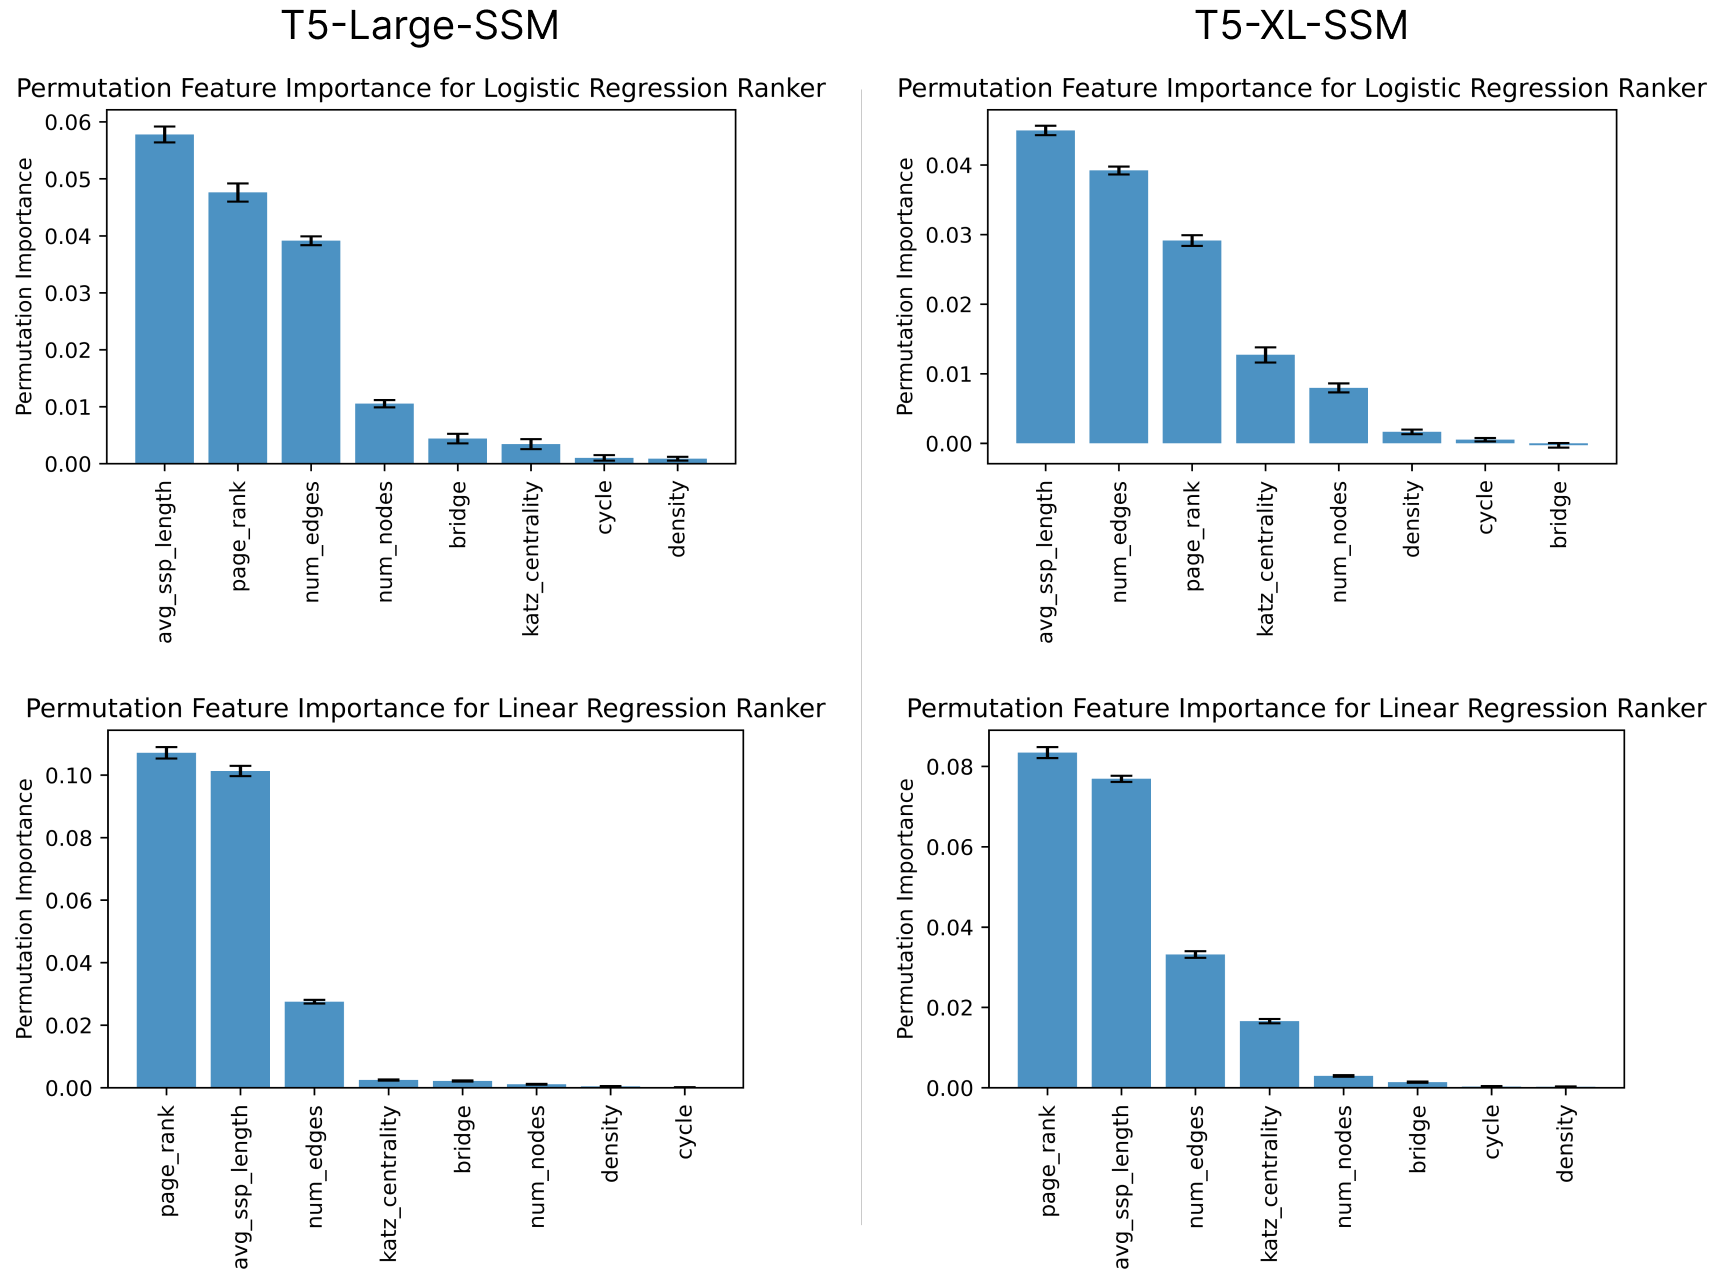
\includegraphics[width=\textwidth]{kg_path_fusion/feature_importance_t5_large_xl.png}
   \caption{Permutation importance of graph features for Linear and Logistic Regression rankers on answer candidates generated by T5-Large-SSM and T5-XL-SSM. The analysis reveals the relative contribution of each feature to the model's performance.}
   \label{fig:controllable_fusion:feature_importance_t5_large_xl}
\end{figure}

\begin{figure}[htb]
   \centering
   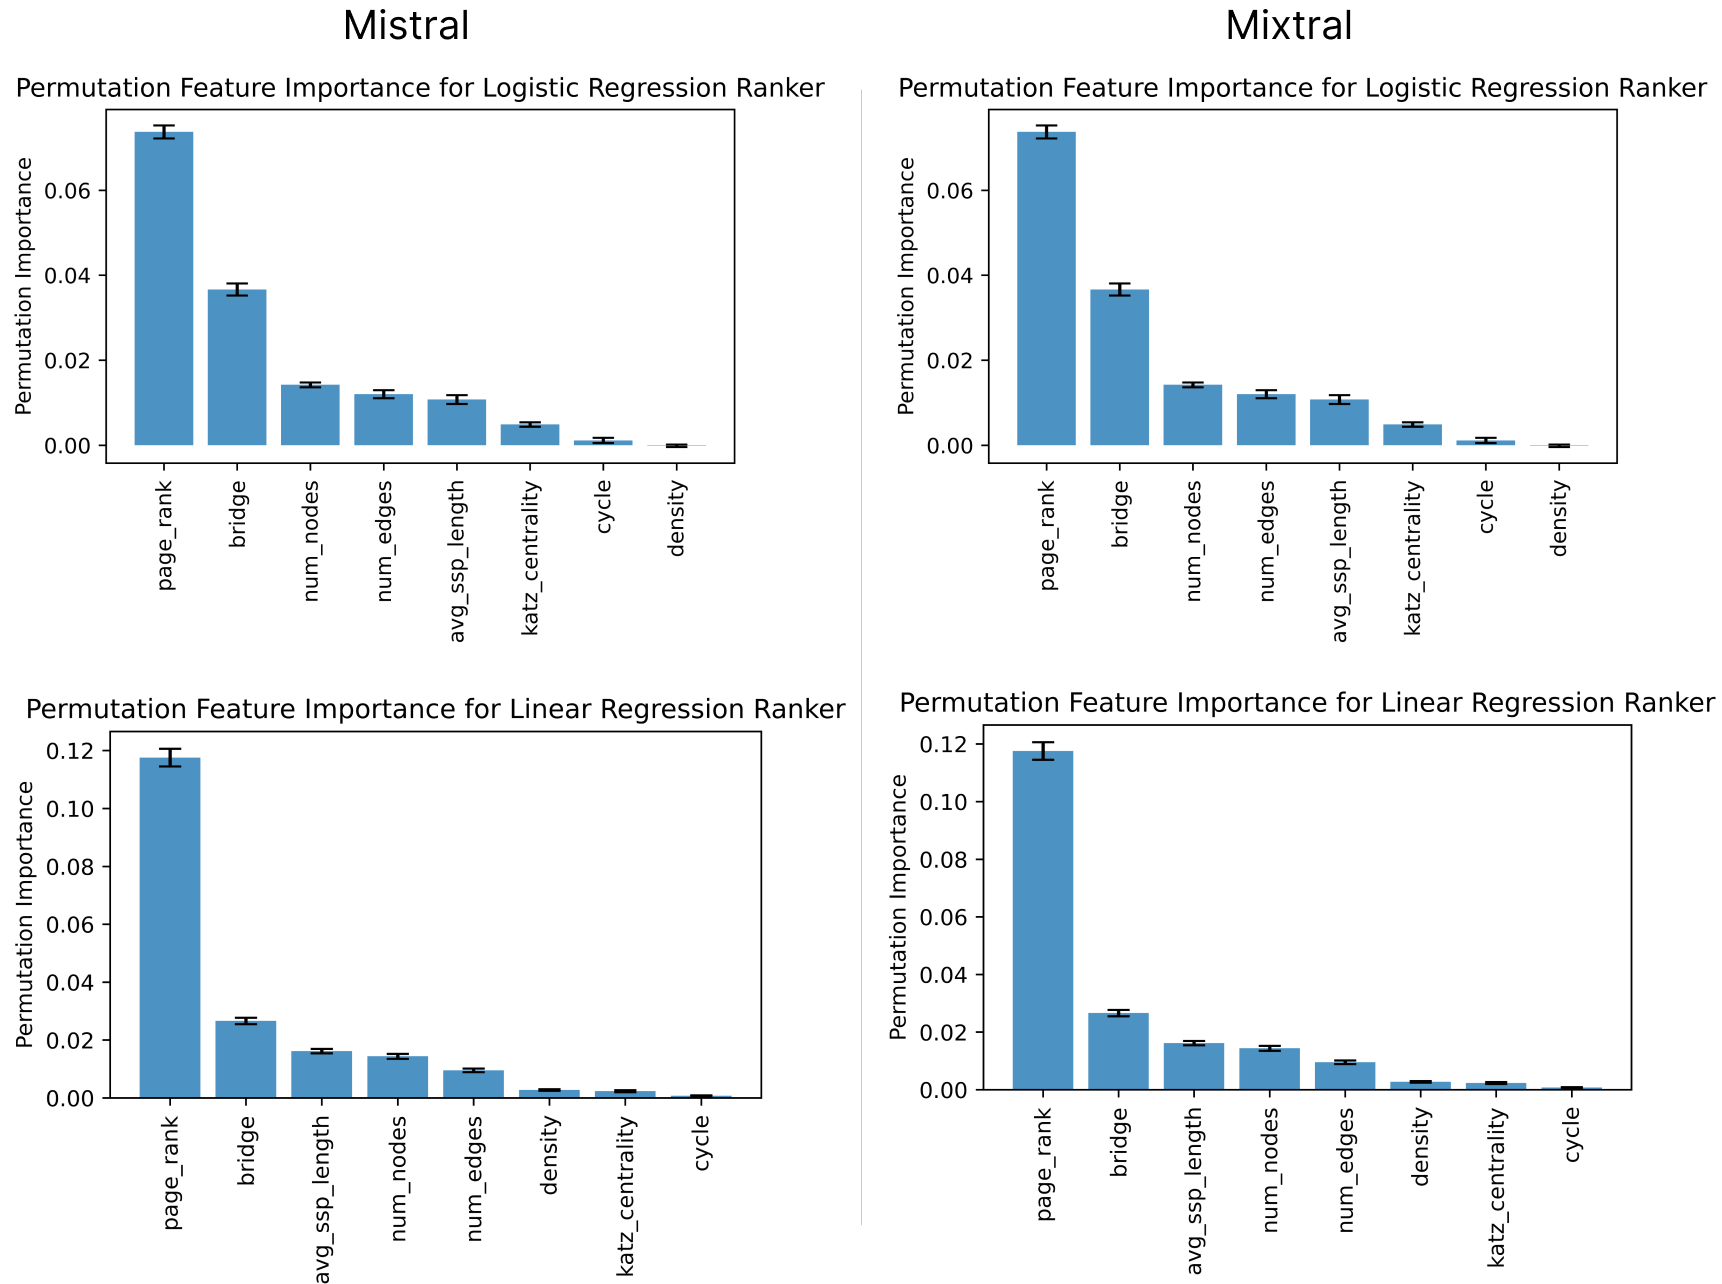
\includegraphics[width=\textwidth]{kg_path_fusion/feature_importance_mistral_mixtral.png}
   \caption{Permutation importance of graph features for Linear and Logistic Regression rankers on answer candidates generated by Mistral and Mixtral. The results show how different features contribute to the ranking performance for these state-of-the-art models.}
   \label{fig:controllable_fusion:feature_importance_mistral_mixtral}
\end{figure}

Lastly, we conducted a comprehensive analysis of feature importance for our gradient-boosting rankers, specifically focusing on the CatBoost implementation. This analysis is particularly interesting because CatBoost offers unique capabilities in handling diverse feature types. Unlike traditional regression-based rankers, CatBoost natively supports a wide range of feature formats:

\begin{enumerate}
    \item Numerical features, which represent continuous values
    \item Categorical features, which represent discrete categories
    \item Text features, which contain natural language content
    \item Embedding features, which capture semantic information in vector form
\end{enumerate}

This versatility in feature handling is particularly advantageous for our task, as it allows us to process embedding features without the need to split them into individual components, unlike the regression-based approaches discussed earlier. This capability makes it possible to assess the importance of both graph-based features and embedding-like features simultaneously, providing a more holistic view of feature contributions.

However, we encountered a limitation in CatBoost's native embedding support. The framework uses order target encodings for embedding features, which introduces ambiguity in the interpretation of results. Additionally, this embedding algorithm is not widely adopted in the natural language processing community, making it less suitable for our specific use case. Given our focus on end-user requirements and practical applicability, we decided to exclude this component from our analysis.

The results of our feature importance analysis for CatBoost rankers are presented in two figures: Figure~\ref{fig:controllable_fusion:feature_importance_t5_large_xl_catboost} shows the analysis for T5-Large-SSM and T5-XL-SSM models, while Figure~\ref{fig:controllable_fusion:feature_importance_mis_mix_catboost} presents the results for Mistral and Mixtral models.

\begin{figure}[htb]
   \centering
   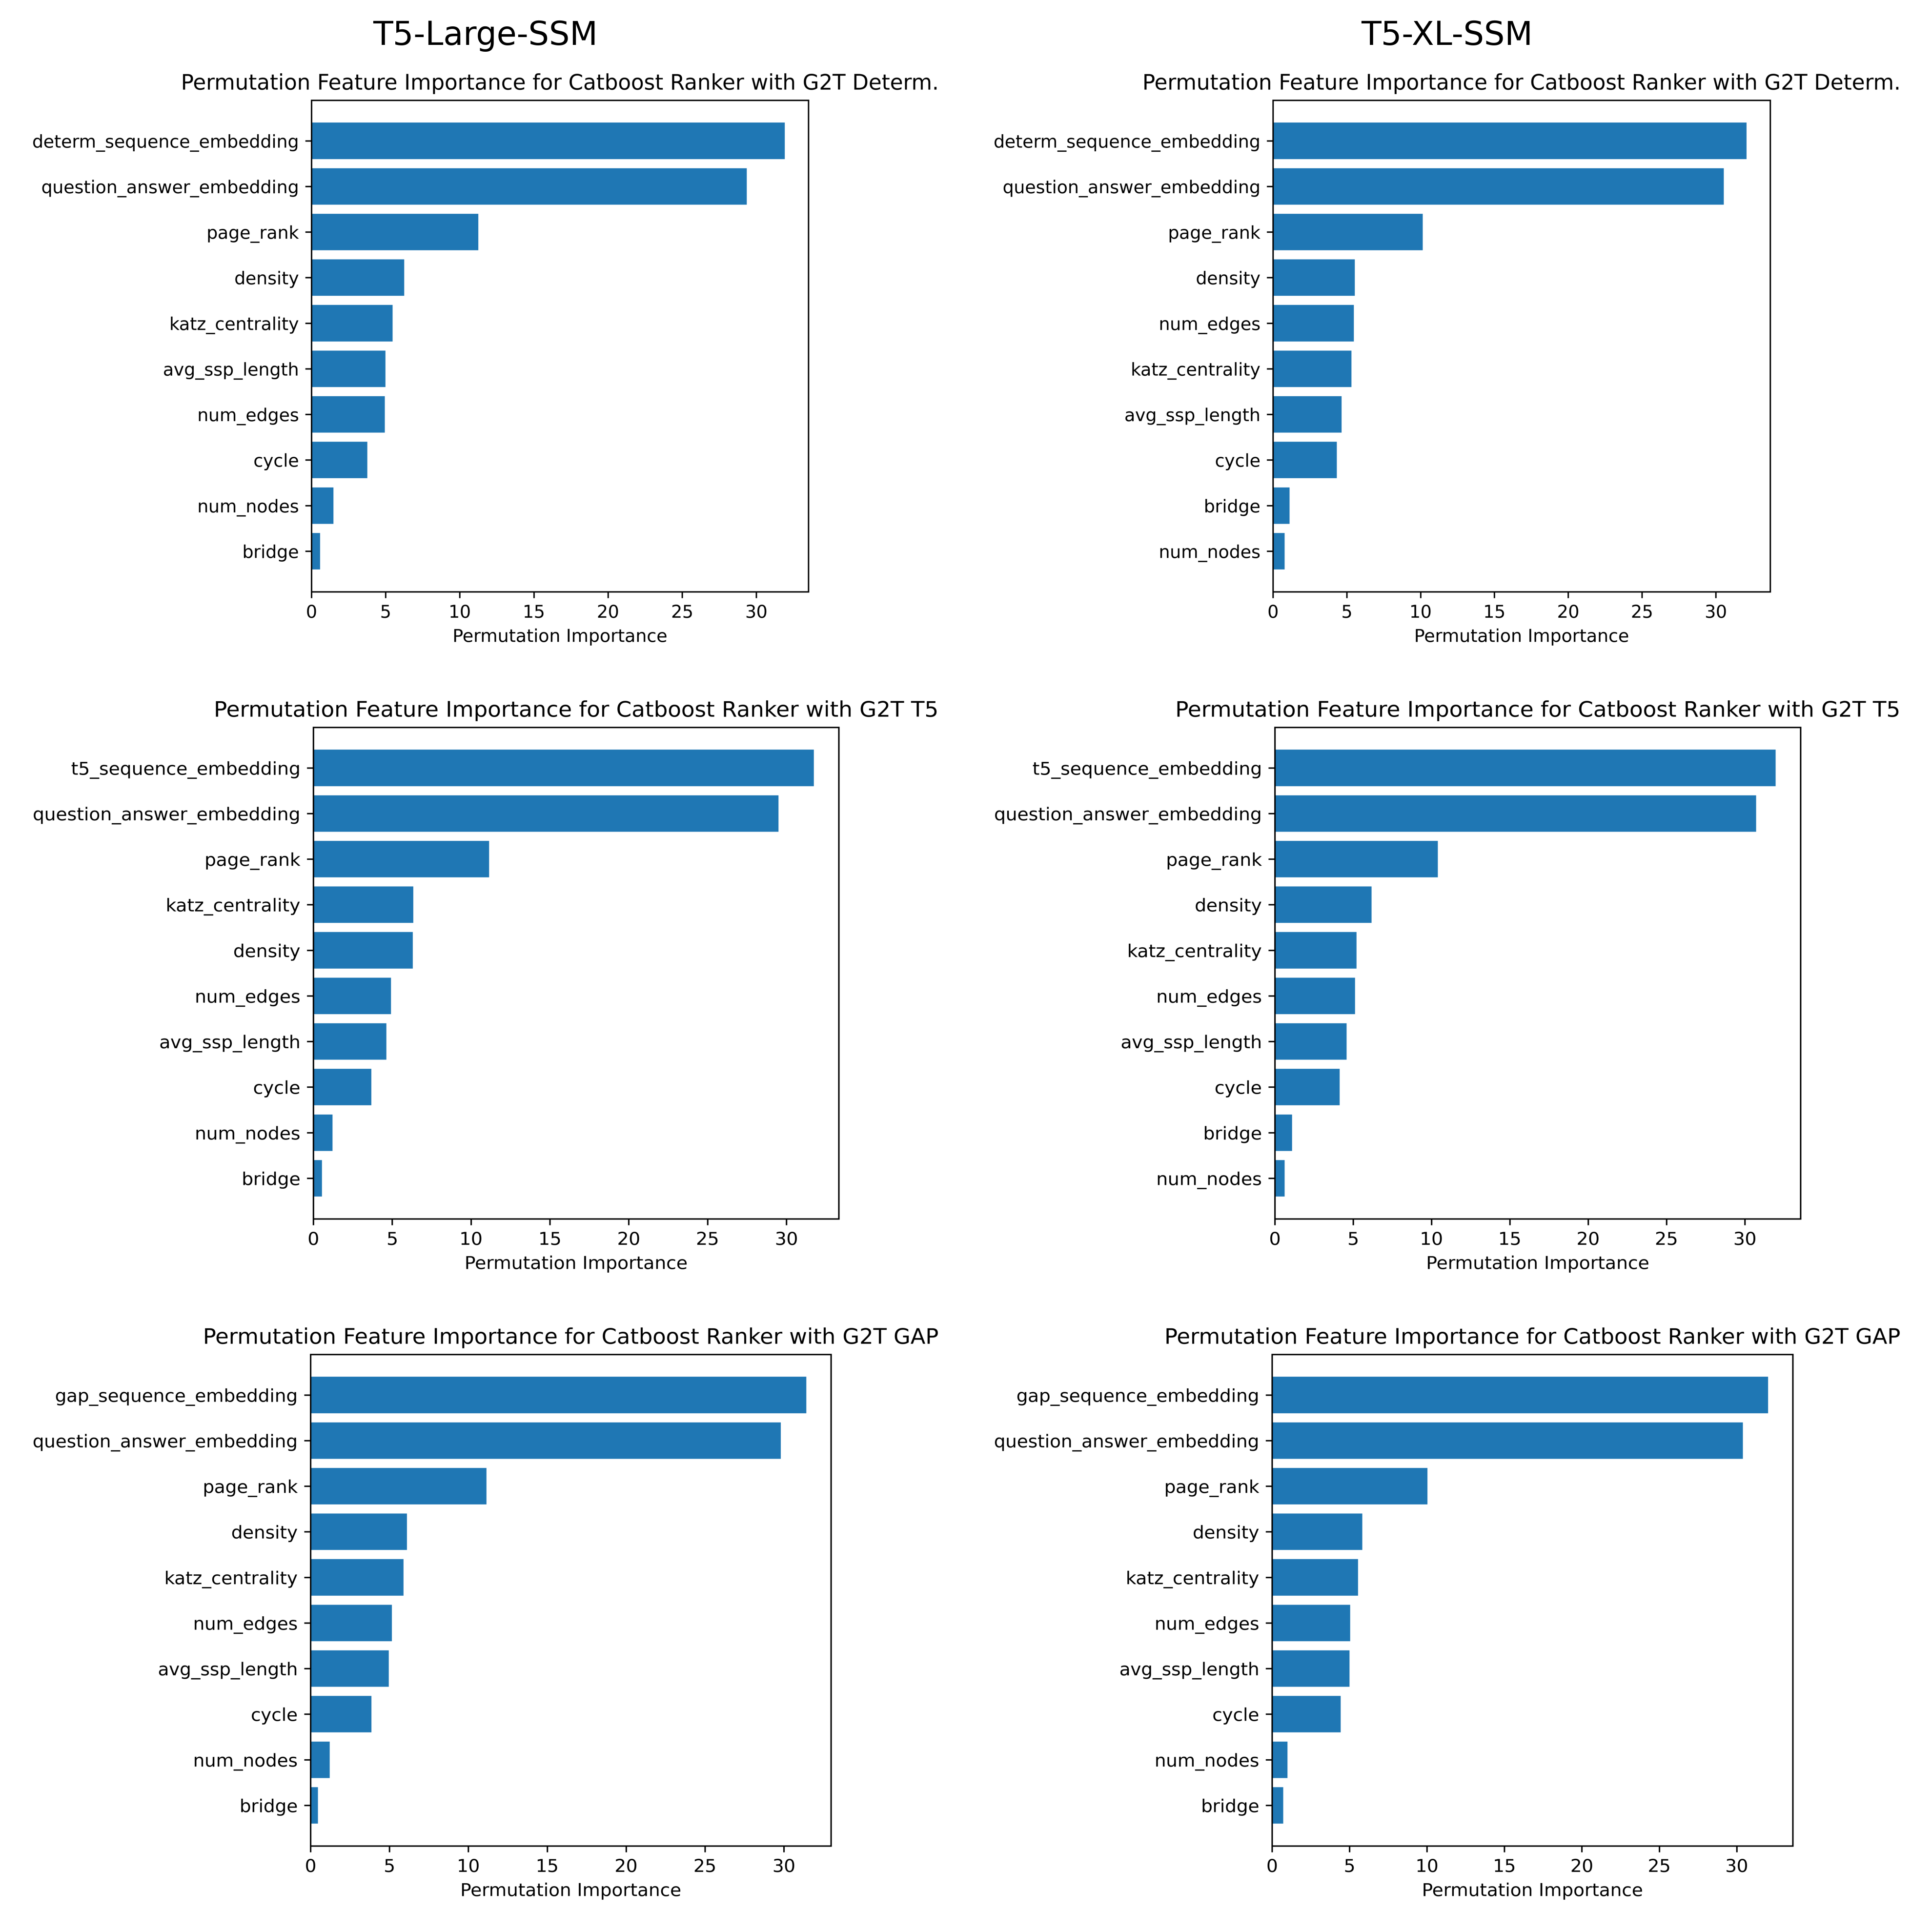
\includegraphics[width=\textwidth]{kg_path_fusion/t5xl_large_catboost.png}
   \caption{Permutation importance of graph, text, and Graph2Text features for CatBoost rankers on answer candidates generated by T5-Large-SSM and T5-XL-SSM. The analysis reveals the relative contribution of different feature types to the model's performance.}
   \label{fig:controllable_fusion:feature_importance_t5_large_xl_catboost}
\end{figure}

\begin{figure}[htb]
   \centering
   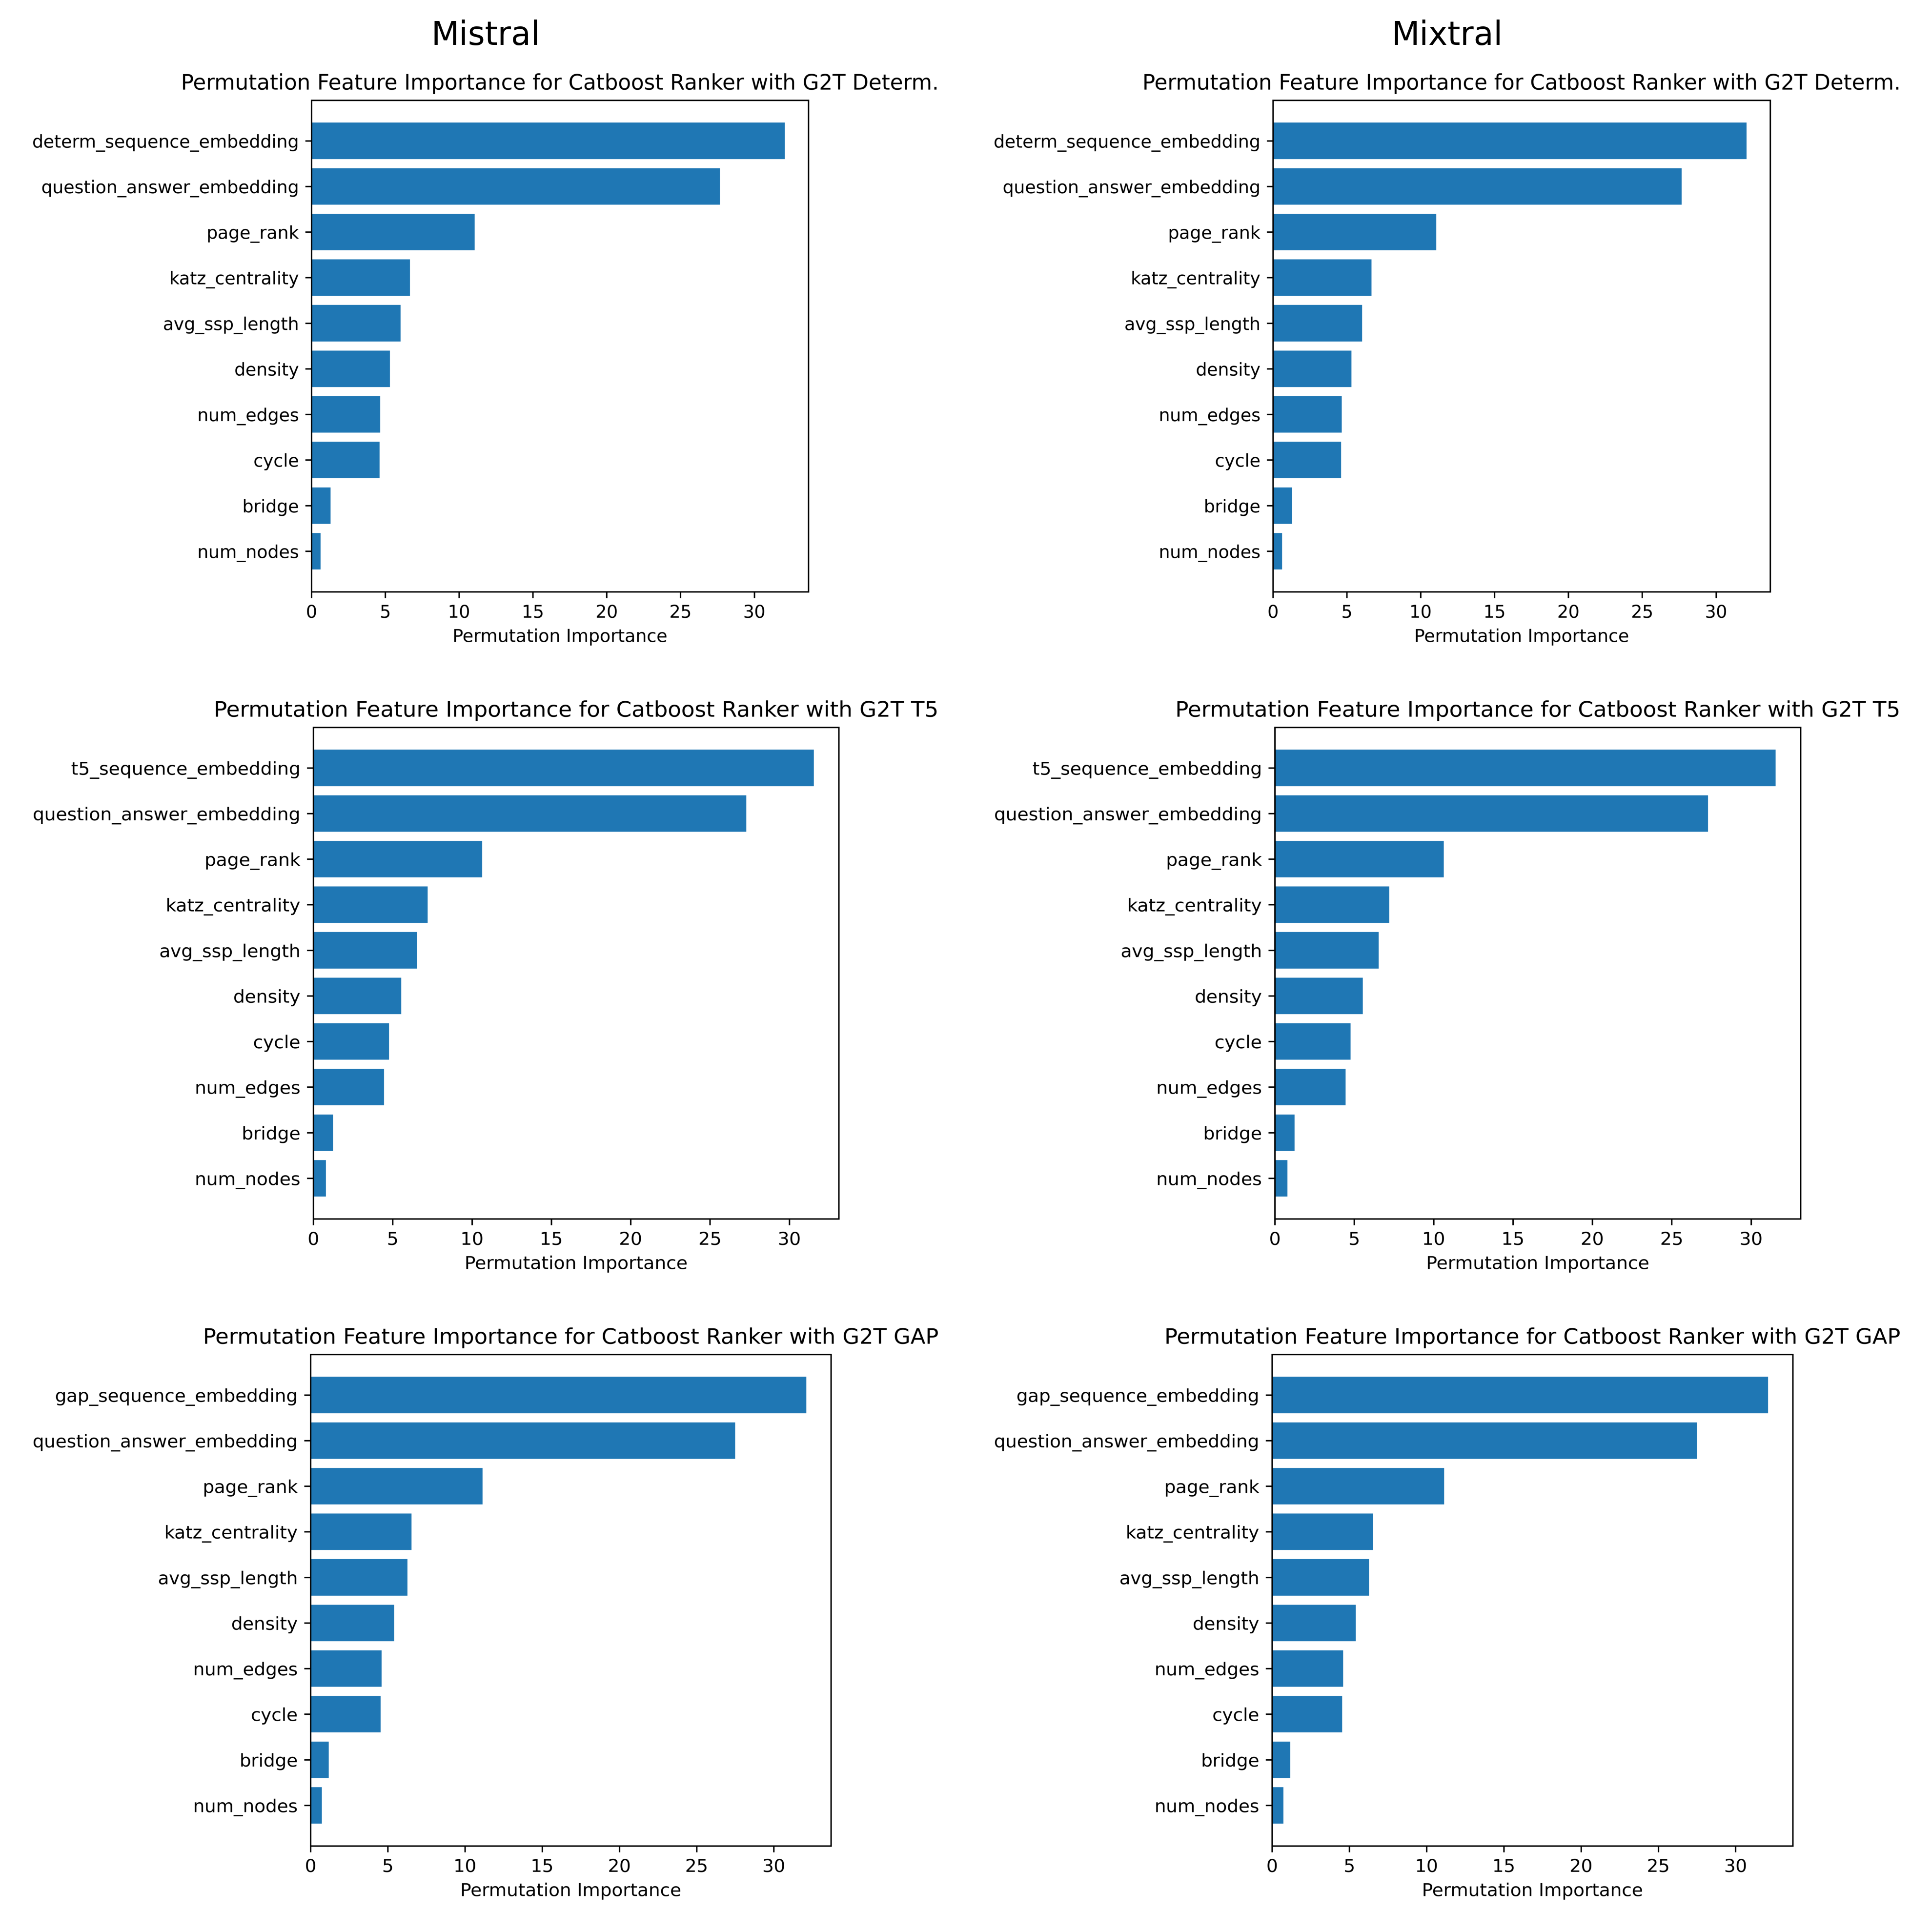
\includegraphics[width=\textwidth]{kg_path_fusion/mistral_mixtral_catboost.png}
   \caption{Permutation importance of graph, text, and Graph2Text features for CatBoost rankers on answer candidates generated by Mistral and Mixtral. The results demonstrate how different feature types contribute to the ranking performance for these state-of-the-art models.}
   \label{fig:controllable_fusion:feature_importance_mis_mix_catboost}
\end{figure}

A detailed examination of the results reveals several significant patterns:

\begin{enumerate}
    \item \textbf{Dominance of Text Features}: The Graph2Text sequence and text features consistently demonstrate the highest importance across all models. This finding strongly supports our earlier observations about the effectiveness of text-based features in the reranking process. The inclusion of initial questions in the feature set appears to be particularly crucial for the ranker's performance.
    
    \item \textbf{Graph Feature Importance}: Among the graph-based features, PageRank emerges as a consistently important factor for both T5-based models and the more recent Mistral/Mixtral models. This observation reinforces the value of PageRank in both classical graph classification tasks and Knowledge Graph Question Answering (KGQA) applications. Other notable graph features include:
    \begin{itemize}
        \item Graph density, which measures the connectivity of the subgraph
        \item Katz centrality, which captures the influence of nodes in the graph
        \item Average shortest path length between question entities and answer candidates
    \end{itemize}
    
    \item \textbf{Model-Specific Variations}: The importance of features varies between different model types, with some features showing higher importance for T5-based models compared to Mistral/Mixtral, and vice versa. This variation suggests that different language models may benefit from different feature combinations.
\end{enumerate}

These findings have important implications for the design of future reranking systems. The strong performance of text-based features suggests that they should be a core component of any reranking system, while the varying importance of graph features across different models indicates that feature selection should be tailored to the specific characteristics of the underlying language model.

\subsection{Hits@N Evaluation Results}

While Hits@1 provides a valuable metric for assessing the top-ranked answer, it offers only a partial view of the reranking approaches' effectiveness. As discussed in Section~\ref{sec:controllable_fusion:evaluation}, we employ the Hits@N metric to conduct a comprehensive analysis of all rankers and feature sets. This broader evaluation allows us to understand how the reranking process affects the entire sequence of candidate answers, not just the top prediction.

In this subsection, we present a detailed analysis of answer sequences both before and after reranking. Our evaluation encompasses:

\begin{enumerate}
    \item \textbf{Comprehensive Testing}: All proposed methods have been evaluated across different feature combinations and model configurations to ensure robust results.
    
    \item \textbf{Multiple N Values}: We calculate Hits@N for various values of N (specifically N=1, 2, and 3) to capture the performance improvements at the top of the ranked list. This approach helps us understand:
    \begin{itemize}
        \item How quickly the correct answer appears in the ranked list
        \item The distribution of correct answers across different positions
        \item The overall effectiveness of the reranking process
    \end{itemize}
    
    \item \textbf{Model Comparisons}: We analyze the performance of different reranking approaches, including:
    \begin{itemize}
        \item Initial predictions from the base language models
        \item Baseline reranking methods
        \item Our proposed approaches with various feature combinations
    \end{itemize}
\end{enumerate}

The detailed results for all combinations of answer candidate sources (T5-Large-SSM, T5-XL-SSM, Mistral, and Mixtral), reranking models, and feature sets are presented in Tables~\ref{tab:controllable_fusion:t5_large_ssm_all_results}, \ref{tab:controllable_fusion:t5_xl_ssm_all_results}, \ref{tab:controllable_fusion:mistral_all_results}, and~\ref{tab:controllable_fusion:mixtral_all_results}. These tables provide a granular view of the Hits@1, Hits@2, and Hits@3 scores, demonstrating the potential of utilizing subgraphs to rerank LLM responses. Moreover, these results underscore the importance of accurately transferring all relevant information from the subgraph to the reranking model. Consequently, the outcomes of this process significantly depend on the quality of the Graph2Text process.

Figure~\ref{fig:controllable_fusion:hit_at_n_plot_all} presents a visual summary of the most significant findings from our comprehensive evaluation, illustrating the overall trends. The results demonstrate several key patterns:

\begin{enumerate}
    \item \textbf{MPNet Superiority}: The reranking approach using MPNet with text and Graph2Text features consistently outperforms both the initial predictions and baseline models. This improvement is particularly notable in the critical Hits@1 metric, where the correct answer appears as the top prediction more frequently.
    
    \item \textbf{Size-Independent Improvement}: The quality enhancement in Hits@1 answers is observed consistently across different language model sizes. This suggests that our reranking approach is robust and effective regardless of the underlying model's complexity.
    
    \item \textbf{Progressive Enhancement}: The improvements in performance are not limited to the top-ranked answer. The reranking process enhances the overall quality of the answer sequence, making it more likely for correct answers to appear in higher positions, as evidenced by the Hits@2 and Hits@3 scores.
\end{enumerate}

These findings underscore the effectiveness of our proposed reranking approach and highlight the importance of considering the entire answer sequence when evaluating question-answering systems. The consistent improvements across different model sizes and the enhanced quality of the top-ranked answers demonstrate the practical value of our methodology.

\begin{figure}[htbp]
   \centering
   \includegraphics[width=0.99\textwidth]{kg_path_fusion/hit_at_n_plot_all.pdf}
   \caption{Comparison of Hits@N performance across different reranking approaches on the Mintaka dataset. The plot shows the cumulative accuracy (Hits@N) for various values of N, demonstrating the effectiveness of different feature combinations and reranking models. The MPNet-based approach with text and Graph2Text features shows consistent improvement over baseline models and initial predictions, particularly in the critical Hits@1 metric. Results are shown for answers generated using Diverse Beam Search across different language model sizes.}
   \label{fig:controllable_fusion:hit_at_n_plot_all}
\end{figure}

\begin{table}[htbp]
    \caption{Hits@1-3 for all proposed reranking approaches and features after reranking the T5-Large-SSM generated answer candidates.}
    \label{tab:controllable_fusion:t5_large_ssm_all_results}
    \fontsize{9pt}{11pt}\selectfont
    \centering
    \setlength{\tabcolsep}{3pt}
    \begin{tabular}{l p{5cm} c c c}
        \toprule
        \textbf{Reranking Model} & \textbf{Features} & \textbf{Hits@1} & \textbf{Hit@2} & \textbf{Hit@3} \\
        \midrule
        Without reranking & & 0.2395 & 0.3580 & 0.4020 \\
        \cmidrule(lr){1-5}
        Full random & & 0.0278 & 0.0562 & 0.0828 \\
        \cmidrule(lr){1-5}
        Semantic reranking & Text & 0.0298 & 0.0647 & 0.0965 \\
        \cmidrule(lr){1-5}
        \multirow{9}{*}{Linear Regression} & Text & 0.2695 & 0.4502 & 0.5400 \\
        & Graph & 0.2338 & 0.4007 & 0.5000 \\
        & Text + Graph & 0.2953 & 0.4697 & 0.5558 \\
        & G2T (Det. Lin.) & 0.2550 & 0.4262 & 0.5230 \\
        & G2T (T5) & 0.2505 & 0.4230 & 0.5193 \\
        & G2T (GAP) & 0.2393 & 0.4133 & 0.5123 \\
        & Text + Graph + G2T (Det. Lin.) & \textbf{0.3065} & 0.4873 & 0.5755 \\
        & Text + Graph + G2T (T5) & 0.3070 & 0.4835 & 0.5710 \\
        & Text + Graph + G2T (GAP) & 0.3033 & 0.4870 & 0.5728 \\
        \midrule
        \multirow{12}{*}{Logistic Regression} & Text & 0.2605 & 0.4353 & 0.5360 \\
        & Graph & 0.2335 & 0.4040 & 0.4980 \\
        & Text + Graph & 0.2470 & 0.4240 & 0.5218 \\
        & G2T (Det. Lin.) & 0.2440 & 0.4203 & 0.5163 \\
        & G2T (T5) & 0.2313 & 0.4068 & 0.5028 \\
        & G2T (GAP) & 0.2925 & 0.4688 & 0.5625 \\
        & Text + Graph + G2T (Det. Lin.) & \textbf{0.3060} & 0.4873 & 0.5745 \\
        & Text + Graph + G2T (T5) & 0.2794 & 0.4780 & 0.5668 \\
        & Text + Graph + G2T (GAP) & 0.2925 & 0.4688 & 0.5625 \\
        \midrule
        \multirow{12}{*}{CatBoost} & Text & 0.2458 & 0.3753 & 0.4525 \\
        & Graph & 0.1935 & 0.3353 & 0.4238 \\
        & Text + Graph & 0.1975 & 0.3463 & 0.4510 \\
        & G2T (Det. Lin.) & 0.2405 & 0.4178 & 0.5068 \\
        & G2T (T5) & 0.2398 & 0.4025 & 0.4868 \\
        & G2T (GAP) & 0.2395 & 0.3975 & 0.4873 \\
        & Text + Graph + G2T (Det. Lin.) & 0.1808 & 0.3208 & 0.4120 \\
        & Text + Graph + G2T (T5) & 0.1888 & 0.3318 & 0.4233 \\
        & Text + Graph + G2T (GAP) & 0.1915 & 0.3350 & 0.4268 \\
        \midrule
        \multirow{10}{*}{MPNet} & Text & 0.2620 & 0.4380 & 0.5345 \\
        & Text + G2T (Det. Lin.) & 0.3399 & 0.5095 & 0.5900 \\
        & Text + G2T (Det. Lin.) + HL & 0.3105 & 0.4853 & 0.5735 \\
        & Text + G2T (T5) & \textbf{0.3493} & 0.5203 & 0.5945 \\
        & Text + G2T (T5) + HL & 0.3468 & 0.5178 & 0.5938 \\
        & Text + G2T (GAP) & 0.3395 & 0.5080 & 0.5890 \\
        & Text + G2T (GAP) + HL & 0.3435 & 0.5170 & 0.5973 \\
        \bottomrule
    \end{tabular}
\end{table}

\begin{table}[htbp]
    \setlength{\tabcolsep}{3pt}
    \caption{Hits@1-3 for all proposed reranking approaches and features after reranking the T5-XL-SSM generated answer candidates.}
    \label{tab:controllable_fusion:t5_xl_ssm_all_results}
    \fontsize{9pt}{11pt}\selectfont
    \centering
    \begin{tabular}{l p{5cm} c c c}
        \toprule
        \textbf{Reranking Model} & \textbf{Features} & \textbf{Hits@1} & \textbf{Hit@2} & \textbf{Hit@3} \\
        \midrule
        Without reranking & & 0.3042 & 0.4298 & 0.4688 \\
        \cmidrule(lr){1-5}
        Full random & & 0.0235 & 0.0473 & 0.0723 \\
        \cmidrule(lr){1-5}
        Semantic reranking & Text & 0.0245 & 0.0545 & 0.0830 \\
        \cmidrule(lr){1-5}
        \multirow{9}{*}{Linear Regression} & Text & 0.2955 & 0.4763 & 0.4763 \\
        & Graph & 0.2550 & 0.4353 & 0.5285 \\
        & Text + Graph & 0.3003 & 0.4825 & 0.5693 \\
        & G2T (Det. Lin.) & 0.2640 & 0.4480 & 0.5375 \\
        & G2T (T5) & 0.2593 & 0.4438 & 0.5333 \\
        & G2T (GAP) & 0.2563 & 0.4320 & 0.5215 \\
        & Text + Graph + G2T (Det. Lin.) & \textbf{0.3220} & 0.5073 & 0.5915 \\
        & Text + Graph + G2T (T5) & 0.3170 & 0.5035 & 0.5818 \\
        & Text + Graph + G2T (GAP) & 0.3153 & 0.5023 & 0.5793 \\
        \midrule
        \multirow{12}{*}{Logistic Regression} & Text & 0.2850 & 0.4683 & 0.5603 \\
        & Graph & 0.2613 & 0.4385 & 0.5283 \\
        & Text + Graph & 0.3003 & 0.4825 & 0.5693 \\
        & G2T (Det. Lin.) & 0.2598 & 0.4420 & 0.5423 \\
        & G2T (T5) & 0.2538 & 0.4393 & 0.5315 \\
        & G2T (GAP) & 0.2503 & 0.4310 & 0.5218 \\
        & Text + Graph + G2T (Det. Lin.) & \textbf{0.3210} & 0.5025 & 0.5885 \\
        & Text + Graph + G2T (T5) & 0.3080 & 0.4955 & 0.5778 \\
        & Text + Graph + G2T (GAP) & 0.3043 & 0.4908 & 0.5815 \\
        \midrule
        \multirow{12}{*}{CatBoost} & Text & 0.2593 & 0.3985 & 0.4720 \\
        & Graph & 0.2760 & 0.4573 & 0.5433 \\
        & Text + Graph & 0.1950 & 0.3370 & 0.4298 \\
        & G2T (Det. Lin.) & 0.2580 & 0.4218 & 0.5130 \\
        & G2T (T5) & 0.2485 & 0.4158 & 0.5025 \\
        & G2T (GAP) & 0.2590 & 0.4390 & 0.5258 \\
        & Text + Graph + G2T (Det. Lin.) & 0.1738 & 0.3160 & 0.4065 \\
        & Text + Graph + G2T (T5) & 0.1670 & 0.3168 & 0.4048 \\
        & Text + Graph + G2T (GAP) & 0.1660 & 0.3093 & 0.4048 \\
        \midrule
        \multirow{10}{*}{MPNet} & Text & 0.3418 & 0.5185 & 0.5960 \\
        & Text + G2T (Det. Lin.) & \textbf{0.3923} & 0.5648 & 0.6260 \\
        & Text + G2T (Det. Lin.) + HL & 0.3628 & 0.5453 & 0.6175 \\
        & Text + G2T (T5) & 0.3905 & 0.5610 & 0.6183 \\
        & Text + G2T (T5) + HL & 0.3760 & 0.5490 & 0.6160 \\
        & Text + G2T (GAP) & 0.3573 & 0.5315 & 0.6040 \\
        & Text + G2T (GAP) + HL & 0.3675 & 0.5528 & 0.6165 \\
        \bottomrule
    \end{tabular}
\end{table}

\begin{table}[htbp]
    \setlength{\tabcolsep}{3pt}
    \caption{Hits@1-3 for all proposed reranking approaches and features after reranking the Mistral generated answer candidates.}
    \label{tab:controllable_fusion:mistral_all_results}
    \fontsize{9pt}{11pt}\selectfont
    \centering
    \begin{tabular}{l p{5cm} c c c}
        \toprule
        \textbf{Reranking Model} & \textbf{Features} & \textbf{Hits@1} & \textbf{Hit@2} & \textbf{Hit@3} \\
        \midrule
        Without reranking & & 0.4655 & 0.5313 & 0.5590 \\
        \cmidrule(lr){1-5}
        Full random & & 0.0920 & 0.1585 & 0.2165 \\
        \cmidrule(lr){1-5}
        Semantic reranking & Text & 0.0858 & 0.1393 & 0.1790 \\
        \cmidrule(lr){1-5}
        \multirow{9}{*}{Linear Regression} & Text & 0.4760 & 0.5818 & 0.6173 \\
        & Graph & 0.3575 & 0.4918 & 0.5653 \\
        & Text + Graph & 0.4810 & 0.5848 & 0.6193 \\
        & G2T (Det. Lin.) & 0.3960 & 0.5298 & 0.5898 \\
        & G2T (T5) & 0.4013 & 0.5295 & 0.5910 \\
        & G2T (GAP) & 0.3885 & 0.5220 & 0.5845 \\
        & Text + G2T (Det. Lin.) & 0.4860 & 0.5875 & 0.6198 \\
        & Text + G2T (T5) & 0.4825 & 0.5845 & 0.6200 \\
        & Text + G2T (GAP) & 0.4770 & 0.5798 & 0.6180 \\
        \midrule
        \multirow{12}{*}{Logistic Regression} & Text & 0.4730 & 0.5795 & 0.6148 \\
        & Graph & 0.3558 & 0.4925 & 0.5645 \\
        & Text + Graph & 0.4745 & 0.5833 & 0.6200 \\
        & G2T (Det. Lin.) & 0.3970 & 0.5260 & 0.5960 \\
        & G2T (T5) & 0.3985 & 0.5305 & 0.5933 \\
        & G2T (GAP) & 0.3850 & 0.5195 & 0.5878 \\
        & Text + G2T (Det. Lin.) & 0.4790 & 0.5833 & 0.6210 \\
        & Text + G2T (T5) & 0.4745 & 0.5838 & 0.6205 \\
        & Text + G2T (GAP) & 0.4728 & 0.5785 & 0.6183 \\
        \midrule
        \multirow{12}{*}{CatBoost} & Text & 0.3918 & 0.5070 & 0.5708 \\
        & Graph & 0.3633 & 0.4995 & 0.5715 \\
        & Text + Graph & 0.3128 & 0.4443 & 0.5295 \\
        & G2T (Det. Lin.) & 0.3863 & 0.5078 & 0.5770 \\
        & G2T (T5) & 0.4013 & 0.5295 & 0.5910 \\
        & G2T (GAP) & 0.3788 & 0.5098 & 0.5775 \\
        & Text + G2T (Det. Lin.) & 0.2883 & 0.4208 & 0.5163 \\
        & Text + G2T (T5) & 0.2568 & 0.3843 & 0.4958 \\
        & Text + G2T (GAP) & 0.3013 & 0.4393 & 0.5265 \\
        \midrule
        \multirow{10}{*}{MPNet} & Text & 0.5115 & 0.6035 & 0.6273 \\
        & Text + G2T (Det. Lin.) & 0.5008 & 0.5913 & 0.6225 \\
        & Text + G2T (Det. Lin.) + HL & 0.5140 & 0.6013 & 0.6288 \\
        & Text + G2T (T5) & 0.4965 & 0.5913 & 0.6230 \\
        & Text + G2T (T5) + HL & 0.5148 & 0.6003 & 0.6253 \\
        & Text + G2T (GAP) & 0.4918 & 0.5880 & 0.6205 \\
        & Text + G2T (GAP) + HL & 0.5073 & 0.5988 & 0.6250 \\
        \bottomrule
    \end{tabular}
\end{table}

\begin{table}[htbp]
    \setlength{\tabcolsep}{3pt}
    \caption{Hits@1-3 for all proposed reranking approaches and features after reranking the Mixtral generated answer candidates.}
    \label{tab:controllable_fusion:mixtral_all_results}
    \fontsize{9pt}{11pt}\selectfont
    \centering
    \begin{tabular}{l p{5cm} c c c}
        \toprule
        \textbf{Reranking Model} & \textbf{Features} & \textbf{Hits@1} & \textbf{Hit@2} & \textbf{Hit@3} \\
        \midrule
        Without reranking & & 0.5173 & 0.5628 & 0.5735 \\
        \cmidrule(lr){1-5}
        Full random & & 0.0580 & 0.1090 & 0.1455 \\
        \cmidrule(lr){1-5}
        Semantic re-anking & Text & 0.0303 & 0.0550 & 0.0715 \\
        \cmidrule(lr){1-5}
        \multirow{9}{*}{Linear Regression} & Text & 0.4883 & 0.5883 & 0.6188 \\
        & Graph & 0.3698 & 0.4983 & 0.5668 \\
        & Text + Graph & 0.4933 & 0.5913 & 0.6208 \\
        & G2T (Det. Lin.) & 0.4083 & 0.5363 & 0.5913 \\
        & G2T (T5) & 0.4135 & 0.5360 & 0.5925 \\
        & G2T (GAP) & 0.4008 & 0.5285 & 0.5860 \\
        & Text + G2T (Det. Lin.) & 0.4983 & 0.5940 & 0.6213 \\
        & Text + G2T (T5) & 0.4948 & 0.5910 & 0.6215 \\
        & Text + G2T (GAP) & 0.4850 & 0.5850 & 0.6198 \\
        \midrule
        \multirow{12}{*}{Logistic Regression} & Text & 0.4853 & 0.5860 & 0.6163 \\
        & Graph & 0.3680 & 0.4990 & 0.5660 \\
        & Text + Graph & 0.4868 & 0.5898 & 0.6215 \\
        & G2T (Det. Lin.) & 0.4093 & 0.5325 & 0.5975 \\
        & G2T (T5) & 0.4108 & 0.5370 & 0.5948 \\
        & G2T (GAP) & 0.3973 & 0.5260 & 0.5893 \\
        & Text + G2T (Det. Lin.) & 0.4913 & 0.5898 & 0.6225 \\
        & Text + G2T (T5) & 0.4868 & 0.5903 & 0.6220 \\
        & Text + G2T (GAP) & 0.4850 & 0.5850 & 0.6198 \\
        \midrule
        \multirow{12}{*}{CatBoost} & Text & 0.4040 & 0.5135 & 0.5723 \\
        & Graph & 0.3755 & 0.5060 & 0.5730 \\
        & Text + Graph & 0.3250 & 0.4508 & 0.5310 \\
        & G2T (Det. Lin.) & 0.3985 & 0.5143 & 0.5785 \\
        & G2T (T5) & 0.3940 & 0.5143 & 0.5793 \\
        & G2T (GAP) & 0.3910 & 0.5163 & 0.5790 \\
        & Text + G2T (Det. Lin.) & 0.3005 & 0.4273 & 0.5178 \\
        & Text + G2T (T5) & 0.2690 & 0.3908 & 0.4973 \\
        & Text + G2T (GAP) & 0.3135 & 0.4458 & 0.5280 \\
        \midrule
        \multirow{10}{*}{MPNet} & Text & 0.5238 & 0.6100 & 0.6288 \\
        & Text + G2T (Det. Lin.) & 0.5130 & 0.5978 & 0.6240 \\
        & Text + G2T (Det. Lin.) + HL & 0.5263 & 0.6078 & 0.6303 \\
        & Text + G2T (T5) & 0.5088 & 0.5978 & 0.6245 \\
        & Text + G2T (T5) + HL & 0.5270 & 0.6068 & 0.6268 \\
        & Text + G2T (GAP) & 0.5040 & 0.5945 & 0.6220 \\
        & Text + G2T (GAP) + HL & 0.5195 & 0.6053 & 0.6265 \\
        \bottomrule
    \end{tabular}
\end{table}

The results highlight that combinations involving textual representations of subgraphs (Graph2Text sequences) and direct text features, especially when processed by neural rankers like MPNet, are particularly effective. For instance, the MPNet model leveraging ``Text + G2T (T5)'' or ``Text + G2T (Det. Lin.)'' features frequently achieves top performance. Furthermore, even simpler regression-based models show notable gains when provided with richer feature sets combining text, graph, and Graph2Text information, often surpassing the initial LLM performance. This underscores the value of integrating structured knowledge from KGs into the reranking pipeline, leading to more accurate and reliable answer selection in question-answering systems. The consistent uplift in performance, irrespective of the base LLM's scale, further reinforces the general applicability and benefit of these subgraph-based reranking techniques.

\section{ShortPathQA: Dataset for Controllable Fusion Knowledge Graphs and Large Language Models}
\label{sec:controllable_fusion:dataset}

Evaluating the effectiveness of methods that fuse Large Language Models (LLMs) with Knowledge Graph (KG) structures, like the subgraph-based reranking approaches discussed in this chapter, requires specific evaluation resources. While many Knowledge Graph Question Answering (KGQA) datasets exist (see Section~\ref{sec:rw_kgqa} for overview), they often focus on the end-to-end task, involving multiple complex stages like entity linking, relation extraction, and subgraph retrieval from massive KGs. This multi-stage nature makes it difficult to isolate and evaluate the performance of the fusion or reranking component itself, as errors can propagate from earlier stages. Furthermore, variations in how different systems extract subgraphs make direct comparison of subgraph processing or reranking techniques challenging~\cite{DBLP:conf/nldb/SalnikovSPQA25}.

Working directly with large-scale KGs like Wikidata also presents significant engineering challenges for many researchers. Tasks such as accurate entity linking, efficient shortest path calculation over billions of triples, and simply hosting the KG (Wikidata, for example, can require terabytes of RAM for efficient in-memory processing) demand substantial computational resources and specialized expertise. This overhead can divert focus from the core research question of how to best utilize the structural information within a KG once it is identified.

These challenges highlighted the need for a standardized dataset specifically designed to facilitate research on controllable fusion methods. Such a dataset should provide pre-computed, relevant KG subgraphs alongside questions and answer candidates, removing the burden of KG hosting and subgraph retrieval. This allows researchers to concentrate directly on developing and comparing models that reason over or rerank based on the provided graph structures. This motivated us to create and publish the ShortPathQA dataset~\cite{DBLP:conf/nldb/SalnikovSPQA25}, which we describe in the following subsections.

ShortPathQA is the first QA dataset that combines textual questions paired with pre-computed Wikidata KG subgraphs applying a unified yet simple subgraph construction approach. The overview of our dataset creation methodology is presented in Figure~\ref{fig:controllable_fusion:big_pipe}. Overall, three key steps should be highlighted: (1) answer candidate generation using an LM; (2) entity linking for both entities mentioned in a question as well as answer candidates from step (1); (3) KG subgraph retrieval with a unified shortest path methodology applied to all questions within a given questions collection.

The code for this dataset is available at \url{https://github.com/s-nlp/ShortPathQA}.

\subsection{Collection of Questions}\label{subsec:question_collection}

ShortPathQA dataset consists of 2 main parts: 
\begin{itemize}
    \item \textbf{Automatic:} A large collection of questions adopted from Mintaka corpus~\cite{DBLP:conf/coling/SenAS22-mintaka} 
    \item \textbf{Manual:} A small collection of new manually curated questions for detailed testing and analysis. 
\end{itemize}

ShortPathQA dataset in build on the Mintaka~\cite{DBLP:conf/coling/SenAS22-mintaka} question format, where each question is annotated with Wikidata entities mentioned in it. While Mintaka does not guarantee a correct answer to be a Wikidata entities, we a sample a subset of questions whose correct answers are the Wikidata entities. Specifically, we remove all \textit{count} questions based on question types provided in the dataset. 
% We refer to the filtered question subset  of our dataset build upon Mintaka questions as \textit{ShortPathQA}.  
% For questions inherited from Mintaka, we preserve the original train/test split (9,750 and 2,430 questions respectively). We will refer to these subsets as \textit{train set} and \textit{automatic test set}, respectively.

In addition to questions adopted from Mintaka, we release \textit{ShortPathQA Manual test set}, a collection of 350 new questions. For consistency with first part of dataset, each question is formulated based on a reference template question from the original Mintaka.  For instance, given a question \textit{``Who is older, The Weeknd or Drake?''} with answer \textit{Drake (Q33240)}, we construct a novel question \textit{``Who was born earlier, Nikolai Ushin or Yossi Abulafia?''} whose answer is \textit{``Nikolai Ushin (Q20203178)''}. 
For each new question, we ensure that it mentions at least one entity with a valid Wikidata identifier;and one or more correct answers to the new question are Wikidata entities. Both types of entities are linked to Wikidata manually.

For \textit{ShortPathQA Manual} test set,  we manually assess the quality of each new created question by ranking it on a scale from 1 to 5, where 1 is ``the given answer is completely irrelevant for the question'', 5 --- ``the given answer is comprehensive for  the given question''. Moreover, we label each question to the question type according to Mintaka classes. Each question was assigned with two annotators. The Kohen's kappa which represents the annotation agreement is $0.81$ for question type and $0.51$ for question quality, the average quality of the questions is $4.81$.


For each answer candidate $c \in \mathcal{A}_q \cup \mathcal{N}_q$, either correct or incorrect, we present the shortest path Wikidata subgraph $\mathcal{G}(q, c)$ describing the shortest path from each entity from $\mathcal{E}_q$ (mentioned in a question) to candidate entity $c$. A visual representation of this process is provided in Figure~\ref{fig:controllable_fusion:big_pipe}. Candidates generated by language model and linked to entities by Wikimedia provided search API\footnote{\href{https://www.mediawiki.org/wiki/Wikibase/API}{www.mediawiki.org/wiki/Wikibase/API}}. This process was detailed describe in Section~\ref{sec:controllable_fusion:answer_candidate_generation} and Section~\ref{sec:controllable_fusion:subgraph_extract}.


\subsection{Dataset Statistics}

Detailed statistics of the proposed ShortPathQA dataset is summarized in Table~\ref{tab:data_statistics}. As seen from the table, our dataset provides over 143K question-candidate pairs with relevant KG subgraphs covering over 32K unique concepts from the Wikidata KG. Notably, the number of Wikidata nodes being answer candidates (26.1K) is higher then the unique candidate name count (24.7K). This implies that some answer candidates can be indistinguishable between each other from their textual names only and relevant KG subgraphs might help overcome the ambiguity.

\begin{table*}[t!]
\centering
\caption{Detailed statistics of the ShortPathQA dataset, including the number of questions, answers, candidates, Wikidata entities mentioned in questions and answer candidates, as well as shortest path graph sizes. \textbf{Test (A)} and \textbf{Test (M)} stand for automatic and manual test sets, respectively.}
\label{tab:data_statistics}
\resizebox{\textwidth}{!}{
    \begin{tabular}{l|cccc||l|cccc}
        \toprule
        % & \multicolumn{4}{c}{\textbf{Subset}} & &\multicolumn{4}{c}{\textbf{Candidate graphs statistics}}  \\
        \multicolumn{5}{c||}{\textbf{Question \& candidate statistics}} & \multicolumn{5}{c}{\textbf{Candidate graphs statistics}}  \\
        \cmidrule{1-5} \cmidrule{6-10}
        \textbf{Statistics} & \textbf{Train} & \textbf{Test (A)} & \textbf{Test (M)} & \textbf{Total} & \textbf{Statistics} & \textbf{Train} & \textbf{Test (A)} & \textbf{Test (M)} & \textbf{Total} \\ \midrule
        \textbf{Questions} & 9,750 & 2,430 & 350 & 12,526 & \textbf{Nodes} & 371,372 & 46,757 & 17,058 & 435,187 \\
        % \multicolumn{5}{c}{\textbf{Answer candidates}} \\
        % \midrule
        \textbf{Candidates} & 123,666 & 15,577 & 3,818 & 143,061 & \textbf{Unique nodes} & 25,457 & 9,867 & 4,895 & 32,226 \\
        % \textbf{Candidate names} & 19,956 & 7,789 & 2,979 & 24,773 \\
        \textbf{Unique names} & 19,956 & 7,789 & 2,979 & 24,773 & \textbf{Avg. \# nodes} & 3 & 3 & 4.47 & 3.04  \\
        % \cmidrule{1-5}\cmidrule{6-10}
        \multicolumn{5}{c||}{\textbf{Covered Wikidata nodes}} & \textbf{Edges} & 423,552 & 53,461 & 21,557 &  498,570  \\
        % \cmidrule{1-5}
        \textbf{Mentioned} & 4,456 & 1,679 & 497 & 5,401 & \textbf{Edge types} & 593 & 450 & 318 & 635 \\
        \textbf{Candidate} & 20,856 & 8,025 & 3,278 & 26,169 & \textbf{Avg. \# edges} & 3.42 & 3.43 & 5.65 & 3.49  \\
        \bottomrule
    \end{tabular}
}
\end{table*}

\subsection{Baseline Evaluation}

To motivate usage of our dataset, we evaluate the performance of the different KGQA approaches on our dataset: (i) zero-shot LLM prediction; (ii) supervised finetuning of LLMs, both an encoder-only Transformer~\cite{DBLP:conf/nips/VaswaniSPUJGKP17} and modern LLM decoder-only model LLaMA3-8b-Instruct~\cite{DBLP:journals/corr/abs-2407-21783-llama3}; (iii) positive/negative class constant; (iv) random baseline. For the first approach, we employ GPT4o, GPT4o mini, and LLaMA3-8b-Instruct models and experiment with adding graph information to the prompt. For the second approach, we adopt the graph linearization approach of~\cite{DBLP:journals/corr/abs-2310-02166} to create a textual representation of an input graph with candidate answers highlighted by special separator tokens. We present both of them in the subsections below.

\subsubsection{Supervised Fine-tuning}
As supervised fine-tuning, we adopt MPNet\footnote{\href{https://huggingface.co/sentence-transformers/all-mpnet-base-v2}{huggingface:sentence-transformers/all-mpnet-base-v2}}~\cite{DBLP:conf/nips/Song0QLL20} and LLaMA3-8B-Instruct~\cite{DBLP:journals/corr/abs-2407-21783-llama3} to encode both questions and linearized subgraphs. The task is formulated as a binary classification: given a question $q$, answer candidate $c$, and KG subgraph $\mathcal{G}(q, c)$, a model has to identify $c$ is a correct answer for $q$. 
We experiment with two input types: (i) \textbf{No Graph}: a model is passed with textual information only: $q\,[SEP]\,c$; (ii) \textbf{With Graph}: a model can reason over graph $\mathcal{L}(q, c)$ to answer observed question: $q\, [SEP] \mathcal{L}(q, c)$. The linearization $\mathcal{L}(q, c)$ of graph $\mathcal{G}(q, c)$ is obtained iteratively by traversing and linearizing individual edges while moving from the mentioned entities $\mathcal{E}_q$ to the answer candidate $c$. 
Each edge $(h, r, t)$ is linearized as $"h, r, t"$. If either $h=c$ or $t=c$, they are additionally emphasized with separator tokens  ``[SEP]'' for the MPNet model: e.g., ``$[SEP]\,h\,[SEP],\,r,\,t$'' if $h=c$. 

For supervised baselines, we use 10\% random questions as validation set for tuning hyper-parameters.
We train each supervised for 10 epochs with a batch size of 32 and learning rate of 1e-5 using Adam optimizer~\cite{DBLP:journals/corr/KingmaB14}. For prediction, we load the model weights from the best epoch in terms of validation F1-score.

The LLaMA3-8B-Instruct model was fine-tuned in a chat format that accepts system messages with short instructions and user messages with questions, answers, and, for the version that accepts subgraphs, a graph in linearized format without tokens. It was trained on 1 epoch of the training dataset. 

\subsubsection{Zero-shot Evaluation}

For zero-shot LLM-based baselines, we ask a model to select correct answers for a question $q$ from the given candidate list $C_q$. If multiple candidates have a matching textual name, we append edge types leading to each candidate $c$ in graph $\mathcal{G}(q, c)$. For example, for the question \textit{"Which film directed by James Cameron became the highest-grossing movie of all time?"} with two candidates answers named "Titanic": (i) \textit{1997 film by James Cameron} and (ii) \textit{1953 film by Jean Negulesco} the candidates are (i) \textit{Titanic (director)} and (ii) \textit{Titanic (original language of performance work)}, respectively. 

Prompt template for all models presented in Table~\ref{tab:controllable_fusion:shortpathqa:prompt_with_subgraph}. For \textbf{No KG} version, we did not used Graph part of user prompt, system prompt was simple instuction: \textit{You are a helpful assistant that verifies answers to questions.}. We employ the OpenAI LLMs\footnote{\href{https://chat.openai.com}{chat.openai.com}} (versions \textit{o3-mini}, \textit{GPT-4o} and \textit{GPT-4o mini}) and LLaMA3-8B-Instruct\footnote{\href{https://huggingface.co/meta-llama/Meta-Llama-3-8B-Instruct}{huggingface:meta-llama/Meta-Llama-3-8B-Instruct}}.

\begin{table*}[htb]
    \caption{LLM prompt to LLaMA3-8b-Instruct, o3-mini, GPT-4o and GPT-4o-mini when given additional subgraph information.}
    \label{tab:controllable_fusion:shortpathqa:prompt_with_subgraph}
        \centering
        \resizebox{\textwidth}{!}{
        \begin{tabular}{>{\raggedright\arraybackslash}p{0.99\textwidth}}
            \toprule
            \makecell[c]{\textbf{System}} \\ \hline
            You are an AI assistant tasked with evaluating the correctness of answers to questions based on 
            provided graph information. The graph consists of triplets in the format (subject, property, 
            object) that demonstrate the shortest path between the question entity and the answer entity.
            \par
            Your role is to:
            \par
              1. Analyze the question and the provided answer carefully.\par
              2. Examine the graph triplets to find connections between the question entity and the answer
                 entity.\par
              3. Evaluate if the shortest path in the graph supports the given answer.\par
              4. Consider that some paths may appear unrelated to the question at first glance but could 
                 still lead to the correct answer.\par
              5. Conclude whether the answer is correct, partially correct, or incorrect based on the graph
                 information.\par
              6. If the answer is incorrect or partially correct, suggest the correct answer based on the 
                 graph data.\par
              7. Provide a short answer.
            \par
            Remember to be thorough in your analysis and clearly communicate your thought process. Your goal 
            is to provide an accurate assessment of the answer's correctness while considering all relevant 
            information from the graph. \\
            \hline
            \makecell[c]{\textbf{User}} \\ \hline
            f"Question: \{q\}\par
            Graph: \{linearize\_graph(g, a, sep\_token=' ')\}\par
            Answer: \{a\} Is this answer correct? Respond with Yes or No:" \\
            \bottomrule
        \end{tabular}
        }
\end{table*}


\subsubsection{Experimental Results}

Evaluation results in terms of positive class precision, recall and F1-score are presented in Table~\ref{tab:controllable_fusion:shortpathqa:res_baselines}. Based on our experiments, GPT-4o is the best model for QA without using subgraphs.

\begin{table*}[ht!]
    \caption{Evaluation results on ShortPathQA test set. Precision, recall, and F1-score are calculated for positive class. o3-mini used with low reasoning effort. The best set-up for each backbone LM is highlighted with \textbf{bold}. The best overall F1-score for each test set is \underline{underlined}.}
    \label{tab:controllable_fusion:shortpathqa:res_baselines}
    \centering
    \resizebox{\textwidth}{!}{
    \begin{tabular}{lcccccc}
        \toprule
        
        \multirow{2}{*}{\textbf{Model setup}} & \multicolumn{3}{c}{\textbf{Automatic Test Set}} & \multicolumn{3}{c}{\textbf{Manual Test Set}} \\ \cmidrule{2-4} \cmidrule{5-7}
        
        & \textbf{Precision}  & \textbf{Recall} & \textbf{F1-score} & \textbf{Precision}  & \textbf{Recall} & \textbf{F1-score}   \\
        \midrule
        Negative class constant & 0.0 & 0.0 & 0.0 & 0.0 & 0.0 & 0.0 \\
        Positive class constant & 0.148 & 1.0 & 0.257 & 0.094 &  1.00 & 0.172 \\
        Random baseline & 0.148 & 0.5 & 0.228 & 0.094 &  0.5 & 0.158 \\
        \midrule
        \multicolumn{7}{c}{\textbf{Supervised evaluation}} \\
        
        
        \midrule
        MPNet (no KG)  & 0.503 & \textbf{0.639} & 0.563  &
        0.167 & 0.507 & 0.251  \\
        MPNet (with KG)  & \textbf{0.609} & 0.631 & \textbf{0.620}  & \textbf{0.275} & \textbf{0.515} & \textbf{0.359}  \\\hline
            
            
        LLaMA3-8b-Instruct \textbf{FT} (no KG)         & 0.689 & 0.751 & 0.719 & 0.507 & 0.713 & 0.593 \\
        LLaMA3-8b-Instruct \textbf{FT} (with KG) & \textbf{0.707} & \textbf{0.755} & \textbf{0.730} & \textbf{0.561} & \textbf{0.749} & \textbf{0.642} \\
        
        \midrule
        \multicolumn{7}{c}{\textbf{Zero-shot evaluation}} \\ \midrule
        
        LLaMA3-8b-Instruct (no KG)                  & 0.432 & \textbf{0.649} & \textbf{0.519} & \textbf{0.376} & 0.749 & \textbf{0.500} \\
        LLaMA3-8b-Instruct (with KG)             & \textbf{0.460} & 0.341 & 0.392 & 0.352 & \textbf{0.783} & 0.486 \\ \hline
        
        GPT4o~mini (no KG)        & \textbf{0.727} & \textbf{0.671} & \textbf{0.698} & \textbf{0.574} & \textbf{0.752} & \textbf{0.652}  \\
        GPT4o~mini (with KG) & 0.653 & 0.544 & 0.594 & 0.561 & 0.705 & 0.625 \\ \hline
        
        
        
        o3-mini (no KG)        & \textbf{0.605} & \textbf{0.805} & \textbf{0.691} & \textbf{0.639} & 0.830 & \textbf{0.723} \\
        o3-mini (with KG)      & 0.493 & 0.804 & 0.612 & 0.520 & \textbf{0.872} & 0.651 \\ \hline
        
        GPT4o (no KG)              & \textbf{0.771} & \textbf{0.769} & \textbf{\underline{0.770}} & \textbf{0.678} & \textbf{0.856} & \textbf{\underline{0.757}} \\
        GPT4o (with KG)      & 0.759 & 0.662 & 0.707 & 0.652 & 0.830 & 0.730 \\ %\hline
        \bottomrule
    \end{tabular}
    }
\end{table*}

The improvement in tuning the LLaMA model has shown that even simple subgraphs can be beneficial for enhancing an LLM's reasoning abilities. The improvement of F1-score on manual test set is notably higher (4.9\%) than on automatic test set (1.1\%). Given a higher graph sizes in the manual part, we assume that relevant KG subgraphs are more crucial for reasoning on complex questions requiring multi-hop reasoning rather than 1-hop reasoning. Compared to zero-shot set-up, LLaMA-3b demonstrates a 14.2\% F1 improvement with graph-aware supervision. While LLMs have bigger capacity to memorize simple factual knowledge, the improvement when for small MPNet encoder when provided a graph is even more substantial: 5.7\% and 10.8\%, on automatic and manual test sets, respectively. Similarly to results observed on LLaMA, the observed F1-score improvement is more significant on more challenging manual test set.

While supervised evaluation results prove that KG subgraphs provide essential factual information that can boost question answering performance, all three LLMs show degraded performance when given the subgraphs. For some reason, the provided subgraphs-aware prompts turned out to be misleading with an F1 decreases of 2.7\%, 2.7\%, and 1.4\% for GPT4o, GPT4o mini, and LLaMA3-8b on the manual test set, respectively. It follows that LLMs are unable to handle additional factual data and hypothesize that more thorough prompt engineering is required.
    
    

\section{Conclusion}
\label{sec:controllable_fusion:chapter_conclusion}

This chapter has presented a comprehensive investigation into leveraging Knowledge Graph (KG) subgraphs for the reranking of answers generated by Large Language Models (LLMs) in the context of Question Answering (QA). We introduced a methodology centered on extracting pertinent subgraphs connecting question entities to candidate answers, followed by the derivation of diverse feature sets—spanning graph-based metrics, textual features, and various Graph2Text (G2T) sequence representations (Deterministic, T5, and GAP).

A systematic evaluation was conducted, employing a range of reranking models from simpler regression-based approaches and CatBoost to more sophisticated neural architectures like MPNet. The empirical results, detailed through extensive Hits@N analyses (Tables~\ref{tab:controllable_fusion:t5_large_ssm_all_results}-\ref{tab:controllable_fusion:mixtral_all_results} and Figure~\ref{fig:controllable_fusion:hit_at_n_plot_all}), consistently demonstrated that the integration of subgraph-derived features significantly enhances answer selection accuracy across various base LLMs (T5-Large-SSM, T5-XL-SSM, Mistral, and Mixtral).

To support such focused evaluations and alleviate the engineering burdens of KG processing, this chapter also introduced the ShortPathQA dataset (Section~\ref{sec:controllable_fusion:dataset}). By providing pre-computed subgraphs for questions derived from Mintaka and a new manually curated set, ShortPathQA offers a standardized benchmark for developing and testing KG-LLM fusion techniques, as demonstrated by the baseline evaluations presented.

Key findings from this chapter include the superior performance of neural rankers, particularly MPNet, when utilizing textual representations of subgraphs, such as G2T sequences combined with the original question context. The feature importance analysis further illuminated the consistent contribution of certain graph metrics like PageRank, while also highlighting the overall dominance of text-based features. Moreover, the study underscored the nuanced performance differences between G2T techniques like T5 and GAP, linking these to their ability to preserve entity information and avoid hallucinations, which directly impacts downstream reranking efficacy.